\documentclass[11pt, a4paper, english]{article}

\usepackage[english]{babel}
\usepackage{BA_Titelseite}

\author{Ayushi XXX}
\geburtsdatum{XX. XXXXXXX XXXX}
\geburtsort{XXXXXXX, XXXXXXXXX}
\date{17 September 2024}
\betreuer{Betreuer: Prof. Dr. Philipp Hieronymi}
\zweitgutachter{Zweitgutachter: Dr. Tingxiang Zou}
\institut{Mathematisches Institut}
\title{Bridging Model Theory and Machine Learning}
\ausarbeitungstyp{Bachelorarbeit Mathematik}

\usepackage[T1]{fontenc}
\usepackage[utf8]{inputenc}
\usepackage[style=alphabetic]{biblatex}
\addbibresource{literature.bib}
\usepackage{amsmath}
\usepackage{amssymb}
\usepackage[thref, standard, amsmath]{ntheorem}
\usepackage[dvipsnames]{xcolor}
\usepackage{csquotes}
\usepackage[colorlinks=true, allcolors=BlueViolet]{hyperref}
\usepackage[capitalise]{cleveref}
\usepackage{mathtools}
\usepackage{marginnote}
\usepackage{enumitem}
\setlist[enumerate]{label={\alph*)}}
\renewcommand*{\marginfont}{\footnotesize\normalfont}
\usepackage{outlines}
\usepackage{tikz}
\usetikzlibrary{shapes,arrows}
\usepackage{tikz-qtree}

%%%%%%%%% mathematical bold  %%%%%%%%%%%%%%%%%

\newcommand{\bA}{\mathbb{A}}
\newcommand{\bB}{\mathbb{B}}
\newcommand{\bC}{\mathbb{C}}
\newcommand{\Cs}{\bC^\times}
\newcommand{\bD}{\mathbb{D}}
\newcommand{\bE}{\mathbb{E}}
\newcommand{\F}{\mathbb{F}}
\newcommand{\bF}{\mathbb{F}}
\newcommand{\bG}{\mathbb{G}}
\newcommand{\bH}{\mathbb{H}}
\newcommand{\bI}{\mathbb{I}}
\newcommand{\bJ}{\mathbb{J}}
\newcommand{\bK}{\mathbb{K}}
\newcommand{\bL}{\mathbb{L}}
\newcommand{\bM}{\mathbb{M}}
\newcommand{\N}{\mathbb{N}}
\newcommand{\bO}{\mathbb{O}}
\newcommand{\bP}{\mathbb{P}}
\newcommand{\bp}{\mathbb{p}}
\newcommand{\Q}{\mathbb{Q}}
\newcommand{\R}{\mathbb{R}}
\newcommand{\bS}{\mathbb{S}}
\newcommand{\bT}{\mathbb{T}}
\newcommand{\bU}{\mathbb{U}}
\newcommand{\bV}{\mathbb{V}}
\newcommand{\bW}{\mathbb{W}}
\newcommand{\bX}{\mathbb{X}}
\newcommand{\bY}{\mathbb{Y}}
\newcommand{\Z}{\mathbb{Z}}

%%%%%%%%% calligraphic %%%%%%%%%%%%%%%%%%%%%%%

\newcommand{\mc}[1]{\mathcal{#1}}
\newcommand{\cA}{\mathcal{A}}
\newcommand{\cB}{\mathcal{B}}
\newcommand{\C}{\mathcal{C}}
\newcommand{\cD}{\mathcal{D}}
\newcommand{\cE}{\mathcal{E}}
\newcommand{\cF}{\mathcal{F}}
\newcommand{\cG}{\mathcal{G}}
\newcommand{\cH}{\mathcal{H}}
\newcommand{\cI}{\mathcal{I}}
\newcommand{\cJ}{\mathcal{J}}
\newcommand{\cK}{\mathcal{K}}
\newcommand{\cL}{\mathcal{L}}
\newcommand{\cM}{\mathcal{M}}
\newcommand{\cm}{\mathcal{m}}
\newcommand{\cN}{\mathcal{N}}
\newcommand{\cO}{\mathcal{O}}
\newcommand{\cP}{\mathcal{P}}
\newcommand{\cQ}{\mathcal{Q}}
\newcommand{\cR}{\mathcal{R}}
\newcommand{\cS}{\mathcal{S}}
\newcommand{\cT}{\mathcal{T}}
\newcommand{\cU}{\mathcal{U}}
\newcommand{\cV}{\mathcal{V}}
\newcommand{\cW}{\mathcal{W}}
\newcommand{\cX}{\mathcal{X}}
\newcommand{\cY}{\mathcal{Y}}
\newcommand{\cZ}{\mathcal{Z}}

%%%%%%%%% mathematical fraktur  %%%%%%%%%%%%%%

\newcommand{\mf}[1]{\mathfrak{#1}}
\newcommand{\fb}{\mathfrak{b}}
\newcommand{\fc}{\mathfrak{c}}
\newcommand{\fA}{\mathfrak{A}}
\newcommand{\fB}{\mathfrak{B}}
\newcommand{\fC}{\mathfrak{C}}
\newcommand{\fD}{\mathfrak{D}}
\newcommand{\fE}{\mathfrak{E}}
\newcommand{\fF}{\mathfrak{F}}
\newcommand{\fG}{\mathfrak{G}}
\newcommand{\fH}{\mathfrak{H}}
\newcommand{\fI}{\mathfrak{I}}
\newcommand{\fJ}{\mathfrak{J}}
\newcommand{\fK}{\mathfrak{K}}
\newcommand{\fL}{\mathfrak{L}}
\newcommand{\fm}{\mathfrak{m}}
\newcommand{\fN}{\mathfrak{N}}
\newcommand{\fO}{\mathfrak{O}}
\newcommand{\fp}{\mathfrak{p}}
\newcommand{\fQ}{\mathfrak{Q}}
\newcommand{\fq}{\mathfrak{q}}
\newcommand{\fR}{\mathfrak{R}}
\newcommand{\fS}{\mathfrak{S}}
\newcommand{\fT}{\mathfrak{T}}
\newcommand{\fU}{\mathfrak{U}}
\newcommand{\fV}{\mathfrak{V}}
\newcommand{\fW}{\mathfrak{W}}
\newcommand{\fX}{\mathfrak{X}}
\newcommand{\fY}{\mathfrak{Y}}
\newcommand{\fZ}{\mathfrak{Z}}

%%%%%%%%%    math operators    %%%%%%%%%%%%%%%

\let\leq=\leqslant
\let\geq=\geqslant 

%%%%%%%%%    further commands  %%%%%%%%%%%%%%%
% Outlines configurations

\makeatletter
% the outline environment provides commands \1..\4 for
% introducing items at level 1..4, and \0 for normal paragraphs
% within the outline section.
\renewenvironment{outline}[1][]{%
  \ifthenelse{\equal{#1}{}}{}{\renewcommand{\ol@type}{#1}}%
  \ol@z%
  \newcommand{\0}{\ol@toz\ol@z}%
  \newcommand{\1}{\vspace{\dimexpr\outlinespacingscalar\baselineskip-\baselineskip}\ol@toi\ol@i\item}%
  \newcommand{\2}{\vspace{\dimexpr\outlinespacingscalar\baselineskip-\baselineskip}\ol@toii\ol@ii\item}%
  \newcommand{\3}{\vspace{\dimexpr\outlinespacingscalar\baselineskip-\baselineskip}\ol@toiii\ol@iii\item}%
  \newcommand{\4}{\vspace{\dimexpr\outlinespacingscalar\baselineskip-\baselineskip}\ol@toiiii\ol@iiii\item}%
}{%
  \ol@toz\ol@exit%
}
\makeatother

%%%%%%%%%    thm environments  %%%%%%%%%%%%%%%
\numberwithin{lemma}{section} 
\numberwithin{theorem}{section} 
\numberwithin{example}{section}

\theoremstyle{plain}
\newtheorem{thm}{Theorem}[section]
\renewtheorem{lemma}[thm]{Lemma}
\renewtheorem{corollary}[thm]{Corollary}

\theorembodyfont{\normalfont}
\renewtheorem{definition}[thm]{Definition}
\renewtheorem{remark}[thm]{Remark}
\renewtheorem{example}[thm]{Example}
\newtheorem{fact}[thm]{Fact}

\usepackage[right=5cm, marginparwidth=4cm, marginparsep=6mm]{geometry}
\usepackage{pgfplots}
\usepackage{nccmath}
\usepackage{dsfont}
\usepackage{csquotes}
\usepackage{tabularx}
\usepackage{layouts}
\usepackage{emptypage}


\newcommand{\notimplies}{\mathrel{{\ooalign{\hidewidth$\not\phantom{=}$\hidewidth\cr$\implies$}}}}
\newcommand\Cfin{\C_{\text{fin}}}
\newcommand\eps{\varepsilon}
\newcommand\samplecomp{N_{\eps,\delta}}
\newcommand\ra{\rightarrow}
\newcommand\VCdim[1]{\operatorname{VCdim}(#1)}
\newcommand\Ldim[1]{\operatorname{Ldim}(#1)}
\newcommand\Xtwo{\prescript{X}{}{2}}
\newcommand\Ytwo{\prescript{Y}{}{2}}
\newcommand\overlinea{\overline{a}}
\newcommand\shatterfunc{\pi_\C}
\newcommand\Lshatterfunc{\rho_\C}
\newcommand\mis{\operatorname{mis}(H,f,\overline{a})}
\newcommand\err{\operatorname{err}_\mu(H,f,\overline{a})}
\newcommand\errNoA{\operatorname{err}_\mu(H,f,-)}
\newcommand\errNoANoF{\operatorname{err}_\mu(H,-,-)}
\newcommand\errNoF{\operatorname{err}_\mu(H,-,\overline{a})}
\DeclareMathOperator{\EX}{\mathbb{E}}
\DeclareMathOperator{\Var}{Var}
\newcommand\symmdiff{\bigtriangleup}
\newcommand\supp{\operatorname{supp}}
\newcommand\dens{\operatorname{dens}}
\newcommand\shelahrank{R^\phi(p)}
\newcommand\shelah[1]{R^\phi(p \land #1)}
\newcommand\Th{\operatorname{Th}}
\newcommand\Adm[2]{\operatorname{Adm}^{#1}_{#2}}
\newcommand{\tF}{\texttt{F}}
\newcommand{\tx}{\texttt{x}}
\newcommand{\ty}{\texttt{y}}
\let\HH\H
\renewcommand\H{\cH}
\renewcommand{\exp}{\mathrm{e}}
\DeclarePairedDelimiter{\ceil}{\lceil}{\rceil}
\DeclareMathOperator*{\argmax}{arg\,max}
\newcommand\ACF{\operatorname{ACF}}
\newcommand\DCF{\operatorname{DCF}}
\let\emptyset\varnothing
\let\phi\varphi
\newcommand\cFx{\cF_x}
\newcommand\cFnotx{\cF_{\overline{x}}}
\newcommand\rhox{\rho_x}
\newcommand\rhoNotx{\rho_{\overline{x}}}
\newcommand\ops{\operatorname{op}_s}
\def\outlinespacingscalar{0.8}
\newcommand{\fa}{\mathfrak{a}}

\newif\ifshowmarginnotes
%%% \showmarginnotestrue to show 
\showmarginnotesfalse

%%% custom margin note for attribution
\newcommand{\contribution}[1]{%
  \ifshowmarginnotes
    \marginnote{\textcolor{gray}{#1}}
  \fi
}

\begin{document}

\maketitle

% \pagenumbering{gobble}
% \section*{Acknowledgments}
% My journey in mathematics began in the summer of 2020, many years after I last had to pick up pen and paper and solve an equation in high school. I had always enjoyed challenges, and the prospect of tackling difficult problems excited me. However, personal circumstances meant that I could never afford the education I wanted. It wasn't until six years after leaving my home country and a year into my new job that I finally decided to pursue what I had long desired. 

% Now, more than four years later, I've learned to respect and appreciate mathematics for its incredible complexity and its abstract beauty, a perspective only so many people get to experience. This journey has been incredibly challenging, many times pushing me to the absolute limits of my abilities---and beyond---and for that, I'm grateful. I've grown and hardened not only intellectually, but also personally. While I'm proud of what I've accomplished, I'm also relieved that my time in Bonn is coming to an end. 

% I am grateful to my employer, NRW.BANK, and my manager, Klaus-Martin Karl, for giving me the opportunity to pursue my academic dreams. It was their support that made it possible in the first place. 

% I am grateful to Lisanne Göbel for guiding me through many of the difficult obstacles during my studies. It is my working alliance with them that has enabled me to complete this thesis. It really means a lot to me. 

% Most importantly, I would like to thank my wife, Polina. Her emotional support over the past few years has been invaluable to me. She has been my emotional bedrock. Beyond her help with my studies, I am grateful for the wonderful life we share together.

% \newpage\phantom{blabla}\newpage

\setcounter{tocdepth}{3}
\tableofcontents


\subsection*{Conventions}
Throughout the text we make use of shorthand notation as common in model theory. We denote
\begin{outline}
    \1 the set of integers $\{0,1,\ldots,n-1\}$ as $n$, 
    \1 a finite number $n\in \N$ as $n<\omega$,
    \1 the set of all subsets of $X$ of size $n$ as $\binom{X}{n}$,
    \1 the set of all functions $f:X\ra Y$ as $\prescript{X}{}{Y}$. 
    \0 For example, the set of all functions $f:X \ra \{0,1\}$ is denoted as $\Xtwo$.
    \1 $\log$ denotes the logarithm to the base 2,
\end{outline}
For any set $Y$ there exists only one function $f:\emptyset\ra Y$, also known as the \emph{empty function}.

%I should probably find the exact place where I use it and put it as a footnote.
\clearpage
\newpage\null\thispagestyle{empty}\newpage
\pagenumbering{arabic}

\addcontentsline{toc}{section}{\protect\numberline{}Introduction}
\section*{Introduction}

\begin{outline}
\0 This thesis explores the fascinating connections between two seemingly disparate fields of mathematics and computer science: model theory and machine learning. At first glance, these areas may appear to have little in common --- model theory is a branch of mathematical logic concerned with the formal study of mathematical structures, while machine learning focuses on algorithms that can learn and make predictions from data. However, there are deep and surprising links between fundamental concepts in these domains. 

Our investigation centers on two key relationships:

\1 The connection between Probably Approximately Correct (PAC) learnability in computational learning theory and the model-theoretic notion of NIP (Non-Independence Property) formulas.

\1 The correspondence between online learnability in computational learning theory and stable formulas in model theory.

\0 These connections allow us to bridge abstract logical properties of theories with concrete learnability guarantees for concept classes. By translating between the languages of logic and learning theory, we gain new insights into the theoretical foundations of machine learning and expand our understanding of the expressiveness of logical theories. This thesis is structured in two main parts:

\0 In the first part, we prove the fundamental theorem of PAC learning, which establishes that a concept class is PAC learnable if and only if it has finite Vapnik-Chervonenkis (VC) dimension. We then introduce NIP theories and demonstrate the equivalence between finite VC dimension and the NIP property. 

\0 The second part explores online learning and the Littlestone dimension as a measure of concept class complexity. We present the Standard Optimal Algorithm for online learning and prove its optimality. On the model theory side, we establish the equivalence between finite Littlestone dimension and Shelah's 2-rank. This allows us to show that stable formulas correspond to concept classes with finite Littlestone dimension.

\0 Finally, we illustrate these concepts with several examples of stable theories. These examples demonstrate how model theory provides a rich source of concrete, learnable concept classes.

\0 While a deep understanding of these areas is not required, readers are expected to have some background in key areas. In model theory, familiarity with first-order logic, languages, structures, models and theories is beneficial. Knowledge of key theorems such as the Löwenheim-Skolem theorem and the compactness theorem will be particularly helpful. In probability theory, knowledge of basic concepts including probability spaces, measures, random variables and expectation will be helpful. 

% \0 All contributions are marked according to the official requirements for theses in the bachelor study program Mathematik at the University of Bonn. We indicate the source material in round brackets after theorem or lemma. Margin notes indicate the degree of personal contribution:
%     \1 0 indicates exact copy of the source material,
%     \1 1 indicates minor contribution: worked out details and improved structure and clarity of the argument,
%     \1 2 indicates major contribution: there was a significant amount of work done to extend and explain the argument,
%     \1 3 indicates original contribution.
% \0 In some cases, we will provide a brief explanation of our exact contribution in the margin notes.
\end{outline}

\newpage 

\section{VC dimension and NIP theories}

\subsection{PAC learning framework}

The Probably Approximately Correct (PAC) learning framework, introduced by Leslie Valiant in 1984, provides a formal foundation for analyzing machine learning problems. It offers a mathematical model to quantify when and how learning is possible, bridging the gap between computational learning theory and practical machine learning algorithms.

In the PAC framework, the learner receives a sample of labeled examples $\{(x_i,f(x_i)) : i\in n\}$, where each $x_i$ is drawn independently from $X$ according to the unknown distribution $\mu$, and $f \in \C$ is the ground truth they aim to learn. The learner's goal is to output a hypothesis $h\in\H$ that, with high probability, closely approximates the target concept $f$ on future examples drawn from the same distribution. 

At its core, PAC learning addresses a fundamental question: Under what conditions can a learning algorithm reliably generalize from a finite set of examples to accurately predict outcomes on unseen data? 

\begin{definition}
\contribution{2 --- Synthesized from multiple sources, independently worded.}
\begin{outline}
\0 The framework formalizes this idea by introducing several key components:
    \1 An \emph{input space} $X$ is a set of all possible instances,
    \1 A \emph{concept} $f$ is a binary-valued function $X\rightarrow\{0,1\}$,
    \1 A \emph{concept class} $\C\subseteq \Xtwo$ is a class of concepts,
    \1 A \emph{target concept} $f\in\C$ is the true function to be learned,
    \1 A \emph{hypothesis} $h$ is a function, representing the learner's prediction,
    \1 A \emph{hypothesis class} $\H\subseteq \Xtwo$ is a set of hypotheses $h$,
    \1 A \emph{sample} $S=\{(x_1,f(x_1)),\ldots,(x_n,f(y_n))\}\subseteq (X\times 2)^n$, $n<\omega$, corresponding to the restriction of target function $f$ to $\{x_1,\ldots,x_n\}$. 
    \1 A \emph{hypothesis function} or a \emph{learning function} $H:\Cfin \rightarrow \H$. It represents an algorithm or deterministic procedure, which given a sample $S$ corresponding to the restriction $f|_S\in\Cfin$ outputs a prediction $H(f)$.
        \2 $\Cfin = \{\C|_Y : Y\subseteq X, Y\text{ finite}\}$ represents all possible labeled samples from $X$.   
\end{outline}
\end{definition}

\begin{remark}[Restrictions]
\label{remark:consistentRealizable}
\contribution{2 --- Synthesized from multiple sources, independently worded.}
\begin{outline}     
\0 In this thesis, we focus on PAC learning with two important properties:
    \1 Consistency: A hypothesis $h$ is \emph{consistent} with a labeled sample, if it correctly classifies all instances in that sample. Formally, given a sample $S$, $h$ satisfies $\forall x_i \in S : h(x_i)=f(x_i)$. Similarly, a hypothesis function $H$ is \emph{consistent}, if for all $f\in\C$ and all $S\subseteq X$ finite it holds $\forall x\in S : H(f|_S)(x)=f(x)$. 
    \1 Realizability: This assumes that there exists a hypothesis $h\in\H$ which perfectly classifies all instances, that is $\forall x\in S : h(x)=f(x)$. 
\0 Given our focus on the realizable case, we will assume that the hypothesis class $\H$ is equal to the concept class $\C$. Consequently, we can refine our notation and sometimes write $H:\Cfin \rightarrow \C$ or $H:\Cfin \rightarrow \Xtwo$ in special cases.
\end{outline}
\end{remark}

\begin{definition}[PAC learnability]
\label{def:PAClearnability}
\contribution{2 --- Synthesized from multiple sources, independently worded.}
\begin{outline}
\0 Let $\C$ be a concept class on a set $X$. We say that $\C$ is \emph{probably approximately correct (PAC) learnable} if there exists a hypothesis function $H:\Cfin \rightarrow \Xtwo$ such that:
    \1 For all $\eps, \delta \in (0,1)$, there exists a natural number $\samplecomp < \omega$ satisfying the following condition:
    \1 For all $n \geq \samplecomp$, all $f \in \C$, and all probability measures $\mu$ on $X$ (with the correct sets being $\mu$-measurable),
$$\mu^n(\{\overline{a} \in X^n : \err > \eps\}) \leq \delta$$
    where:
        \2 $\eps\in(0,1)$ is the \emph{accuracy parameter}, specifying the acceptable error rate,
        \2 $\delta\in(0,1)$ is the \emph{confidence parameter} indicating the desired probability of successfull learning,
        \2 $\samplecomp: (0,1)^2\rightarrow \N, (\eps,\delta) \mapsto \samplecomp$ is the \emph{sample complexity function}, which determines the minimum number of examples required to guarantee PAC learning. 
        \2 $\err$ is the error of the hypothesis function $H$ predicting $f$ given sample $\overline{a}=(a_1,\ldots,a_n)$, defined by 
        $$\mu^n(\{x\in X : H(f|_{\overline{a}})(x)\neq f(x)\})$$
\0 This definition ensures that with high probability $(1-\delta)$, the learning function $H$ will produce a hypothesis that is approximately correct (up to an error of $\eps$) when the sample size is at least $\samplecomp$.
\end{outline}
\end{definition}

\subsection{The fundamental theorem of PAC Learning}
\label{section:fdmThmofPAC}

The fundamental theorem of PAC learning, first proven by Blumer, Ehrenfeucht, Haussler and Warmuth in 1989, establishes that a concept class is PAC learnable if and only if it has finite VC dimension. This section presents a complete proof of this theorem.

\subsubsection{VC dimension and shatter function}
\label{subsection:1}

\begin{definition}[VC dimension]
\contribution{1 --- Synthesized from multiple sources, independently worded.}
    Let $X$ be an input space and let $\C\subseteq\Xtwo$ be a concept class on $X$. For any $Y\subseteq X$:
    \begin{outline}
        \1 the \emph{restriction} of $\C$ to $Y$ is $\C|_Y := \{ f|_Y : f\in \C\}$.
        \1 $\C$ \emph{cuts out} $Y$ from $X$ if $\exists f\in\C : f|_X = \mathds{1}_Y$. 
        \1 $\C$ \emph{shatters} $Y$ if $\C|_Y = \Ytwo$ or, equivalently, if $\C$ cuts out every subset of $Y$.
    \0 The Vapnik-Chervonenkis (VC) dimension of $\C$, denoted $\VCdim{\C}$, is defined as $$\sup\{ |Y| : Y\subseteq X \text{ is finite and } \C \text{ shatters } Y\}.$$
    If $\C$ shatters arbitrarily large finite sets, then $\VCdim{\C} = \infty$. If $\C$ shatters no set, then $\VCdim{\C} = -\infty$. A concept class $\C$ is called a \emph{VC class} if it has finite VC dimension.
    \end{outline} 
\end{definition}

\begin{remark}[Learning problems and set systems]
\contribution{3.}
    \label{rem:dualitySetSystems}
    There exists a natural correspondence between learning problems $(X,\C)$ and set systems $(X,\cF)$. Each $f\in \C$ defines a unique set $A_f\subseteq X$ where $A_f = \{ a\in X :f(a)=1\}$. 
    The set system perspective often simplifies proofs and combinatorial arguments, while the function-based view aligns more closely with the learning theory framework. We will sometimes use the notation $(X,\cF)$ interchangeably with $(X,\C)$ in our proofs, as this leads to more concise and intuitive arguments.
\end{remark}

Informally, the VC dimension measures the complexity or expressiveness of a concept class in relation to its domain $X$ by looking at how many points it can label arbitrarily. A higher VC dimension indicates that the concept class can represent more complex decision boundaries.

\begin{example}[Easy]
\contribution{1.}
    Consider $X=\R$ and the class of threshold functions $\C = \{f_a(x) : f_a(x)=1 \text{ if } x \geq a, f_a(x)=0 \text{ if } x < a\}$. This class has VC dimension $2$, since it can shatter any set of two points and cannot shatter any set of three points. Note that the definition of VC dimension requires only one set of maximum size to be shattered.
\end{example}

It is important to note that the VC dimension is not an equivalence.
    \begin{center}
        VC dimension $n$ $\notimplies$ any set of cardinality $n$ can be shattered \\
        VC dimension $n$ $\impliedby$ any set of cardinality $n$ can be shattered
    \end{center}


\begin{example}[Intermediate]
\contribution{2.}
    Consider $X=\R^2$ and the class of half-planes $\C = \{f_{a,b}(x) : f_{a,b}(x) = 1 \text{ if } \langle a,x \rangle \geq b, f_{a,b}(x) = 0 \text{ if } \langle a, x \rangle \leq b \}$. Using elementary geometry (specifically, Radon's theorem), one can prove that $\C$ has VC dimension 3.
\end{example}

\begin{remark}
\contribution{3.}
    Prominent mathematician Terry Tao writes in his \href{https://terrytao.wordpress.com/2007/05/23/soft-analysis-hard-analysis-and-the-finite-convergence-principle/}{blogpost}:
    
    \begin{quote}
        In the field of analysis, it is common to make a distinction between \enquote{hard}, \enquote{quantitative}, or \enquote{finitary} analysis on one hand, and \enquote{soft}, \enquote{qualitative}, or \enquote{infinitary} analysis on the other. \enquote{Hard analysis} is mostly concerned with finite quantities (e.g. the cardinality of finite sets, the measure of bounded sets, the value of convergent integrals, the norm of finite-dimensional vectors, etc.) and their quantitative properties (in particular, upper and lower bounds). \enquote{Soft analysis}, on the other hand, tends to deal with more infinitary objects (e.g. sequences, measurable sets and functions, $\sigma$-algebras, Banach spaces, etc.) and their qualitative properties (convergence, boundedness, integrability, completeness, compactness, etc.). To put it more symbolically, hard analysis is the mathematics of $\eps$, $N$, $O()$, and $\leq$; soft analysis is the mathematics of $0$, $\infty$, $\in$, and $\to$.
    \end{quote}
    
    This distinction also characterizes the approaches to VC dimension in computer science and model theory.

    In computer science, researchers typically employ a quantitative approach to VC dimension. They often seek to determine or estimate the exact VC dimension of concept classes, as this provides explicit bounds on learning complexity. Their proofs typically follow a two-step approach:
    First, they show that any set of cardinality $n+1$ cannot be shattered and then they explicitly shatter a set of cardinality $n$. 

    In contrast, model theorists generally adopt a qualitative approach to VC dimension. Their primary concern is whether the VC dimension is finite or infinite, rather than its exact value. A model theorist might prove that a theory $T$ has finite VC dimension (equivalently, is NIP) without necessarily computing the exact VC dimension of any particular formula in $T$.
\end{remark}

The following example illustrates the \enquote{soft} approach in model theory:

\begin{example}[Hard]
\contribution{3.}
    The theory of real ordered field\footnote{A reader without a background in model theory can safely skip this example until later sections, where we discuss it in detail.} with an exponential function is o-minimal, and thus NIP. This implies that any formula $\phi$ is NIP and the concept class uniformly defined by $\phi$ is a VC class. Such examples provide only qualitative information about the learnability, without specifying the exact VC dimension.
\end{example}

% \begin{remark}[Concept classes vs. definable sets]
%     \label{rmk:setsystemduality}
%     Since we restrict ourselves to concept classes with values in $\{0,1\}$, we can and will sometimes identify functions with their support, since any function is defined by its support and vice versa. A model theorist would say we identify formulas with sets defined by formulas. \textcolor{red}{Should add about CS input space / concept class $X, \C$ vs logic set system two-sorted structure $X, \cF$? Relevant for Ldim equivalence part later...}
% \end{remark}

The next two theorems establish elementary properties of VC dimension. The first theorem demonstrates the monotonicity properties of VC dimension with respect to both the input space and the concept class. 
The second theorem shows how VC dimension changes when concept classes are combined using different Boolean operations. 

\begin{theorem}[Basic properties I]
\label{thm:VCbasic1}
Let $\C \subseteq 2^X$ be a concept class on input space $X$ with $\VCdim{\C}=d<\infty$.
\begin{outline}
    \1[(1)] Any subset of a shattered set $A$ is shattered.
    \1[(2)] For any set $Y$ with $Y \subseteq X$:
    $\VCdim{\C|_Y} \leq \VCdim{\C}$.
    \1[(3)] For any concept classes $\C'$ with $\C' \subseteq \C$:
    $\VCdim{\C'} \leq \VCdim{\C}$.
\end{outline}
\end{theorem}

\begin{proof}
\begin{outline}
\contribution{3 --- Independent proof of widely known properties, warm-up.}
\0 Let $(X,\cF)$ be the set system corresponding to $(X,\C)$ by $\cref{rem:dualitySetSystems}$.
    \1[(1)] Let $B\subseteq A$. To show $B$ is shattered, we need to prove that $\forall S \subseteq B : \exists F \in \cF : F\cap B = S$. Since $B$ is a subset of $A$, $S$ is also a subset of $A$. Since $A$ is shattered by $\cF$, there exists $F\in\cF : F\cap A = S$. Now, $F\cap B = (F\cap A) \cap B = S\cap B = S$. Therefore, we have found $F\in\cF$ such that $F$ cuts out $S$. Since $S$ was arbitrary, this holds for all subsets of $B$. Thus, $B$ is shattered by $\cF$.
    \1[(2)] Let $A\subseteq Y$ be any set shattered by $\cF|_Y$. We need to show that $|A| \leq d$.
    For every subset $S\subseteq A$, there exists a set $(F\cap Y)\in\cF|_Y : (F\cap Y)\cap A = S$. Since $A\subseteq Y$, this implies $(F\cap Y)\cap A = F\cap A = S$. Therefore $A$ is also shattered by $\cF$. Since $\VCdim{\C} = d$, we must have $|A|\leq d$.
    \1[(3)] Let $\cF' \subseteq \cF$ and let $A$ be any set shattered by $\cF'$. Since $\cF'\subseteq \cF$ this automatically implies that $A$ is shattered by $\cF$. Since $\VCdim{\C} = d$, we must have $|A|\leq d$.
\end{outline}
\end{proof}

\begin{theorem}[Basic properties II]
\label{thm:VCbasic2}
Let $X$ be an input space, $f\in\Xtwo$ a function, and $\C_1$ and $\C_2$ concept classes of VC dimension $n_1<\omega$ and $n_2<\omega$. Then the following holds regarding concept classes and their VC dimensions:
\begin{outline}
    \1[(1)] intersection $\C_\cap = \{ f_1 \cdot f_2 : f_1 \in \C_1, f_2 \in \C_2\}$, $\VCdim{\C_\cap} \leq \max \{n_1,n_2\}$,
    \1[(2)] union $\C_\cup= \{f_1+f_2 - (f_1\cdot f_2) : f_1 \in \C_1, f_2 \in \C_2\}$, $\VCdim{\C_\cup} \geq \max \{n_1,n_2\}$
    \1[(3)] negation $\C_\lnot= \{1-f_1 : f_1\in\C_1\}$, $\VCdim{\C_\lnot} =n_1$
    \1[(4)] symmetric difference $\C\symmdiff f= \{|g-f| : g\in\C_1\}$, $\VCdim{\C\symmdiff f} = n_1$
\end{outline}
\end{theorem}
\begin{proof}
\begin{outline}
\contribution{3 --- Independent proof of widely known properties, warm-up.}
\0 Let $(X,\cF_1), (X,\cF_2)$ be the set systems corresponding to $(X,\C_1),(X,\C_2)$. Let $(X,\cF_1\symmdiff B), B=\{x\in X : f(x)=1\}$ be a set system corresponding to $(X,\C\symmdiff f)$. The statements to prove correspond to Boolean operations on $\cF_1$ and $\cF_2$.  
    \1[(1)] By \cref{thm:VCbasic1}(3), $\VCdim{\C_1\cap \C_2} \leq \max \{n_1,n_2\}$. 
    \1[(2)] By \cref{thm:VCbasic1}(3), $\VCdim{\C_1\cup \C_2} \geq \max \{n_1,n_2\}$.
    \1[(3)] Let $A\subseteq X$ of cardinality $n_1$ be shattered by $\C_1$. For every subset $S\subseteq A$, $\exists F\in \cF_1 : F\cap A = S$. This implies $\forall (A\setminus S)\subseteq A, \exists F \in \cF_1 : A \setminus (F\cap A) = A\setminus F = A\setminus S$. Since each $S$ is in one-to-one correspondence with $(A\setminus S)$, $\VCdim{\C_\lnot} = n_1$.
    \1[(4)] Let $A\subseteq X$ of cardinality $n_1$ be shattered by $\C_1$. The proof is a character-building exercise in basic set theory. We show that any two sets in $\cF_1$ cut out the same subset from $A$ if and only if they cut out the same subset in $(\cF_1\symmdiff B)$.
        \2 For any $F_1,F_2 \in \cF_1$, we have:
        \begin{align*}
            F_1 \cap A = F_2 \cap A 
            \iff & F_1 \cap B \cap A = F_2 \cap B \cap A \text{ and } \\
            & F_1\cap (X\setminus B)\cap A = F_2\cap (X\setminus B)\cap A
        \end{align*}
        This equivalence holds because $A$ can be partitioned into $A\cap B$ and $A\cap (X\setminus B)$.
        \begin{align*}
            \iff & (X\setminus F_1) \cap B \cap A = (X\setminus F_2) \cap B \cap A \text{ and } \\
            & F_1 \cap (X\setminus B) \cap A = F_2 \cap (X\setminus B) \cap A
        \end{align*}
        This equivalence holds because membership in $F_1$ completely determines membership in $X\setminus F_1$.
        \begin{align*}
            \iff & 
            \left((X\setminus F_1)\cap B\right) \cup \left(F_1\cap (X\setminus B)\right) \cap A = \\
            & \left((X\setminus F_2)\cap B\right) \cup \left(F_2\cap (X\setminus B)\right) \cap A
        \end{align*}
        This step combines the two conditions using set union. This equivalence holds because the sets $(X\setminus F_1)\cap B$ and $F_1\cap (X\setminus B)$ are disjoint (and similarly for $F_2$).
        \begin{align*}
            \iff & 
            (F_1\symmdiff B)\cap A = (F_2\symmdiff B)\cap A.
        \end{align*}
        The final step uses the definition of symmetric difference. 
        \2 Therefore, $\C_1|_A$ cuts out $2^{n_1}$ subsets from $A$ if and only if $(\C_1\symmdiff f)|_A$ cuts out $2^{n_1}$ subsets from $A$. This implies that they both shatter $A$ and have the same VC dimension.
    % You can align multiples align* with a table: (looks kinda ugly though)
    % \begin{tabularx}{\linewidth}{l@{}c@{}X}
    % $F_1 \cap A = F_2 \cap A$ & $\iff$ & $F_1 \cap B \cap A = F_2 \cap B \cap A$ and \\
    % & & $F_1\cap (X\setminus B)\cap A = F_2\cap (X\setminus B)\cap A $ \\
    % \multicolumn{3}{l}{This equivalence holds because $A$ can be partitioned into $A\cap B$ and} \\
    % \multicolumn{3}{l}{$A\cap (X\setminus B)$.} \\
    %                           & $\iff$ & $(X\setminus F_1) \cap B \cap A = (X\setminus F_2) \cap B \cap A$ and\\
    %                           &        & $F_1 \cap (X\setminus B) \cap A = F_2 \cap (X\setminus B) \cap A$ \\
    % \multicolumn{3}{l}{This step uses the fact that $F\cap B = X\setminus ( (X\setminus F)\cap B)$ for any $F$.} \\
    %                           & $\iff$ & 
    % \end{tabularx}
        % \2 To show that $\VCdim{\C} \leq \VCdim{\C\symmdiff f}$ it suffices to prove that $\pi$ is injective. $S'=(S\setminus B) \cup ((B\setminus S)\cap A)$ satisfies $\pi(S')=S$. 
        % \setlength\delimitershortfall{-1pt}
        % \begin{align*}
        % S'\symmdiff B & = \left(S'\setminus B\right) \cup 
        % \left(B\setminus S'\right) \\
        % & = \left(\left(\left(S\setminus B\right) \cup \left(\left(B\setminus S\right)\cap A\right)\right)\setminus B\right) \cup \left((B\setminus \left((S\setminus B) \cup \left(\left(B\setminus S\right)\cap A\right)\right)\right)\\ 
        % & = \left( S \setminus B\right) \cup \left(B \cap \left(B\setminus\left(B\setminus S\right) \cap A \right)\right) \\
        % & = \left( S \setminus B\right) \cup B \\
        % & = S.
        % \end{align*}
        % \2 To show $\VCdim{\C\symmdiff f} \leq n_1$, note that for any $G \in \C\symmdiff f$, there exists $F \in \C_1$ such that $G = F \symmdiff B$. If a set $A'$ is shattered by $\C\symmdiff f$, then for any $S' \subseteq A'$, there exists $F \in \C_1$ such that $(F \symmdiff B) \cap A' = S'$. This implies $F \cap A' = S' \symmdiff (B \cap A')$, which means $A'$ is shattered by $\C_1$. Therefore, $|A'| \leq n_1$.
        % Combining both inequalities, we conclude $\VCdim{\C\symmdiff f} = n_1$.
\end{outline}
\end{proof}

While VC dimension considers all possible subsets of $X$, it is often useful to analyze how the concept class behaves on subsets of specific sizes. This allows us to examine how the \enquote{shattering power} of the concept class grows as we increase the size of the subsets we consider.

\begin{definition}[Shatter function]
\contribution{0.}
    \label{def:shatterfunc}
    Define the \emph{shatter function} $\shatterfunc(m):\N \ra \N$ as
    $$\shatterfunc(m):= \max \left\{|\C_Y| : Y \in \binom{X}{m}\right\}.$$
\end{definition}  

\begin{lemma}[Sauer-Shelah, 1972]
\marginnote[0cm]{The function $\Phi_n(m)$ counts the number of subsets of an $m$-element set that have size less than or equal to $n$. In other words, it represents the number of subsets of $\{1,2,\ldots,m\}$ with cardinality at most $n$.}
    \label{lemma:Sauer-Shelah}
    Define $\Phi_n(m):=\sum^n_{i=0}\binom{m}{i}$. If $\C$ has VC dimension $n$ and $m>n$, then $\shatterfunc(m) \leq \Phi_n(m)$.
\end{lemma}

There exist numerous proofs and versions of this lemma, which has important applications in model theory, graph theory, computational geometry and other disciplines. We give a proof using the \enquote{shifting} technique commonly used in extremal set theory. 
% https://cse.buffalo.edu/~hungngo/classes/2010/711/lectures/sauer.pdf

\begin{proof}[Lemma 1.5, \cite{Chernikov}]
\begin{outline}
\contribution{1 --- Improved proof structure and clarity.}
\0 We proceed by contradiction. Fix some $m>n$ and suppose $\shatterfunc(m) > \Phi_n(m)$.
    \1 By \cref{def:shatterfunc}, there exists $Y\subseteq X$ with $|Y|=m$ such that $|\C|_Y| = \shatterfunc(m) > \Phi_n(m)$. Since $\shatterfunc(m)$ depends only on the size of $|\C|_Y|\leq 2^Y$, we can without loss of generality assume that: 
        \2 $\C$ is finite with $|\C| = \shatterfunc(m)$,
        \2 $X=\{x_1,\ldots,x_m\}$ with $|X|=m$.
\0 We construct a sequence of concept subclasses $\C_0,\ldots,\C_m$ of $\C$ using a \enquote{shifting} operation. 
    \1 Let $\C_0 := \C$.
%\marginnote[0cm]{Assume $\C_0=\{f\}$ with $f(x_1,x_2,x_3,x_4,x_5)=(1,1,0,1,0)$ or $11010$.\\ 
% $\C_1 = \{01010\}$.\\
% $\C_2 = \{00010\}$.\\
% $\C_3 = \{00010\}$.\\
% $\C_4 = \{00000\}$.\\
% $\C_5 = \{00000\}$.}
    \1 Given $\C_k$, construct $\C_{k+1}$ as follows: 
        \2 For each $f\in\C_k$, if $f(x_{k+1})=1$ and exists $g\not\in\C_k$ such that $g(x_{i\neq k+1})=f(x_{i\neq k+1})$ and $g(x_{k+1})=0$
        % $$\begin{cases}
        %     g(x)=f(x) & x\in \{x_1,\ldots, x_k\} \\
        %     g(x)=0 & x\in \{x_{k+1}\} 
        % \end{cases},$$ 
        then replace $f$ by $g$ in $\C_{k+1}$. Otherwise, keep $f$ in $\C_k$.
    \1 This construction has three key properties:
        \2[(1)] For each $l$, $|\C_k|=|\C_{k+1}|$,
        \2[(2)] If $A$ is shattered by $\C_{k+1}$, then $A$ is shattered by $\C_k$,
        \2[(3)] If $f\in \C_m$, then $\supp(f)$ is shattered by $\C_m$.
    \1 Proofs of properties:
        \2[(1)] Holds by construction: each replacement preserves cardinality.
        \2[(2)] Let $A$ be shattered by $\C_{k+1}$. For any $B\subseteq A$:  
            \3 If $g$ cuts out $B$ and $g\in\C_k$, then $\C_k$ cuts out $B$.
            \3 If $g$ cuts out $B$ but $g\not\in\C_k$, then $g$ must have been added to $\C_{k+1}$ to replace some $f\in\C_k$ during the shifting operation. 
                \4 If $x_{k+1}\not\in A$, then $f\in\C_k$ that $g$ replaced cuts out $B$, since $g|_A=\mathds{1}_B=f|_A$. Thus $\C_k$ cuts out $B$.
                \4 If $x_{k+1}\in A$, then $x_{k+1} \not\in B$ (since $g(x_{k+1})=0$). Since $\C_{k+1}$ shatters $A$, there exists $h\in\C_{k+1}$ cutting out $B\cup \{x_{k+1}\}$. By construction, $h$ must have been in $\C_k$ and $h$ should have been replaced with $h'\not\in \C_k$ cutting out $B$. Since it was not replaced, $h'$ was already in $\C_k$, thus $\C_k$ cuts out $B$. 
                %Since it is both in $\C_k$ and $\C_{k+1}$ and it wasn't swapped out, the only possible combination is if condition $g_h \not\in\C_k$ was not satisfied, so $g_h\in \C_k$ and $g_h$ cuts out $B$ from $A$.
        \2[(3)] Assume $\exists f\in\C_m$ with $\supp(f)$ not shattered by $\C_m$. Then $\exists x_{i+1}\in\supp(f)$ with no $g\in\C_m$ such that $g(x_{i+1})=0$. But $f$ would have been replaced at step $i$ by construction, removing $x_{i+1}$ from $\supp f$. This contradicts the assumption $f\in\C_m$.
\0 It follows from $(2)$ that $\VCdim{\C_m} \leq n$. From $(3)$, no $f\in\C_m$ has $|\supp(f)|>n$. Therefore: 
$\Phi_n(m) \geq |\C_m| \mathrel{\overset{\makebox[0pt]{\mbox{\normalfont\tiny\sffamily $(1)$}}}{=}} 
    |\C| = |\shatterfunc(m)|.$
\end{outline}
\end{proof}

\begin{corollary}[Growth of the shatter function]
\label{cor:shatterfuncGrowth}
\contribution{0.}
Let $\C$ be a concept class of VC dimension $n$. Then,
$$
\shatterfunc(m)
\begin{cases}
    = 2^m & m \leq n \\
    \leq \Phi_n(m) & m > n
\end{cases}
$$
and, in particular, $\shatterfunc(m)\in O(m^n)$.
\end{corollary}

\begin{figure}
    \centering
        \begin{tikzpicture}
        \begin{semilogyaxis}[
            axis lines = left,
            anchor=origin,
            xlabel = \(m\),
            ylabel = {\(\shatterfunc(m)\)},
            xlabel style={at={(axis description cs:1,0.05)},anchor=west},
            ylabel style={at={(axis description cs:0.1,1)},anchor=south,rotate=270},
            xmin= 0, xmax= 15,
            ymin= 0, ymax= 500,
            xtick=\empty,
            ytick=\empty,
            extra x ticks={5},
            extra y ticks={32},
            extra x tick labels={$n$},
            extra y tick labels={$2^n$},
            extra tick style={grid=major, grid style={dashed, black}},
        ]
        \addplot [
            domain=0:5, 
            samples=20, 
            color=blue,
        ]
        {2^x};
        \addplot [
            domain=5:15, 
            samples=20, 
            color=blue,
            ]
            {7+x^2};
        \end{semilogyaxis}
        \end{tikzpicture}
    \caption{A schematic depiction of shatter function growth for a concept class $\C$ with $\VCdim{\C}=n$. The y-axis uses a logarithmic scale. For $m \leq n$, the function grows exponentially as $2^m$. At $m = n$, the function transitions to slower growth, bounded by a polynomial function.}
    \label{fig:enter-label}
\end{figure}

\begin{remark}
\contribution{0.}
    In the special case where $\C = \binom{X}{n}$, this bound is tight for $m>n$.
\end{remark}

\begin{proof}[\cref{cor:shatterfuncGrowth}]
~
\begin{outline}
\contribution{1 --- Added details on growth bound.}
    \1 For $m\leq n$, the bound holds by \cref{thm:VCbasic1}(1).
    \1 For $m>n$, the bound holds by \cref{lemma:Sauer-Shelah}.
    \1 The growth estimate holds due to the following well-known binomial inequality:
    $$\Phi_n(m) = \sum^n_{i=0}\binom{m}{i} \leq  \sum^n_{i=0}\left(\frac{me}{i}\right)^i \leq m^n.$$
    For each term in the sum above, we have
        \begin{align*}
            \binom{m}{i} = \frac{m!}{i! (m-i)!} = \frac{(i+1)(i+2)\ldots(m)}{i!} \leq \frac{m^i}{i!} < \left(\frac{me}{i}\right)^i.
        \end{align*}
\end{outline}
\end{proof}

This result implies that for any given concept class $\C$, its shatter function can only grow either exponentially or polynomially in terms of $m$. As the cardinality of the set increases beyond $n$, the fraction of subsets of the set that can be shattered approaches $0$.

\subsubsection{$\eps$-nets and the VC theorem}
\label{subsection:2}

The next sections lie at the intersection of statistics, probability theory and computer science. Our primary objective is to examine and prove the Vapnik-Chervonenkis (VC) theorem, a fundamental result in statistical learning theory.

To provide additional context, we present a correspondence between some statistical and computational concepts, adapted from a widely-used textbook \enquote{All of Statistics: A Concise Course in Statistical Inference} by Wasserman:

\begin{center}
\begin{tabularx}{\textwidth}{X X X} 
Statistics & Computer Science & Meaning \\
\hline
estimation & learning & using data to estimate an unknown quantity \\
classification & supervised learning & predicting a discrete $Y$ from $X$\\
large deviation bounds & PAC learning & uniform bounds on probability errors
\end{tabularx}
\end{center}

The main goal of this section is the VC theorem, which is a variation on the theme of large deviation bounds. These bounds, which include the well-known Chernoff, Hoeffding, and Markov inequalities, provide estimates for the probability that an average of independent random variables deviates significantly from its expected value.  

To build towards the VC theorem, we will introduce the concept of $\epsilon$-nets. These are subsets of our sample space that, in a sense, approximate the entire space well.

\begin{remark}
\contribution{3.}
    In this section, we let $(X,\cA,\mu)$ denote a probability space. Let $\C$ be a concept class on $X$ so that each $f\in\C$ has $\mu$-measurable support, i.e. for all $f\in\C : \supp(f)\in \cA$. For each $f\in\C$, let $\mu(f)=\mu(\supp(f))=\int_X f d\mu$. In other words, $\mu(f)$ is the $\mu$-probability that, given $a\in X, f(a)=1$. For any $n<\omega$ we consider the product measure of $\mu$ on $X^n$, which we will denote by $\mu^n$. 
\end{remark}

% \begin{definition}[Error function, algorithm]
%     The error of an algorithm $H:\C_{\operatorname{fin}} \ra \Xtwo$ is defined as 
%     $$\errNoA = \mu(\{x\in X : H(f)(x)\neq f(x)\}).$$
%     Put in words, the error is equal to the measure of a set on which our algorithm $f$ is false. This quantifies the probability of our algorithm\ldots \textcolor{red}{I should focus on this and rewrite this soon. This is algorithm error and not function error.}
% \end{definition}

\begin{lemma}[Lemma 2.3.4, \cite{Guingona}]
    \label{lemma:expectedValueOfError}
    Let $\C$ be a PAC learnable concept class on $X$ and let $H$ be a learning function for $f\in \C$ with sample complexity $\samplecomp$. Then, for all $\eps\in(0,1), \delta \in (0,1)$, probability measures $\mu$ on $X$, and $n\geq \samplecomp$,
    $$\EX(\overline{a}\mapsto \err) \leq \delta + \eps(1-\delta).$$
\end{lemma}
\begin{proof}
\contribution{1 --- Improved proof structure and readability.}
    Let $Y_0=\{\overline{a} \in X^n : \err > \eps\}$. Let $Y_1 = X\setminus Y_0$. By definition, since $\C$ is PAC learnable, the probability of sampling $\overline{a} \in Y_0$ with error $> \eps$ is less than $\delta$, so
    \begin{align*}
        \EX(\overline{a}\mapsto \err) & = \int_{X^n}\errNoA d\mu^n \\
        & \leq \int_{Y_0}\errNoA d\mu^n + \int_{Y_1}\errNoA d\mu^n \\
        & \leq  1\cdot \mu^n(Y_0)+\eps \cdot \mu^n(Y_1) \\
        & \leq \delta + \eps (1-\delta).
    \end{align*}
\end{proof}

\begin{definition}[Definition 2.2.6, \cite{Guingona}]
    For $\eps\in(0,1)$, a subset $N \subseteq X$ is called an $\eps$-net for $\C$ if for every $f\in \C$ with $\mu(f)=\mu(\supp(f))\geq \eps$, there exists $a\in N$ such that $f(a)=1$.
\end{definition} 

Intuitively, an $\eps$-net intersects every function $f\in \C$ whose support has $\mu$-measure at least $\eps$. This allows it to serve as an approximation of $X$ with respect to $\C$ capturing all the \enquote{large} sets.

\begin{fact}[Chebyshev's inequality]
\label{fact:Chebyshev}
    If $f:X\rightarrow \R$ is a random variable and $\eps >0$, then 
    $$\mu\left(\{a\in X : |f(a)-\EX(f)|\geq \eps\}\right)\leq \frac{\Var(f)}{\eps^2}.$$
\end{fact}

\begin{lemma}[Lemma 2.2.5, \cite{Guingona}]
    \label{lem:suppfUB}
    Fix $p\in [0,1]$ and finite $n\geq \frac{8}{p}$. Let $(f_0,\ldots,f_{n-1})\in \Xtwo$ such that $\mu(f_i)=p$ for all $i<n$. Then,
    $$\mu\left(\left\{
    (a_1,\ldots,a_n) \in X^n : \sum^n_{i=1} f_i(a_i)\leq \frac{1}{2}np
    \right\}\right) \leq \frac{1}{2}.$$
\end{lemma}
\begin{proof}
\contribution{1 --- Improved proof structure and readability.}
    Define $f:X^n\rightarrow \R$ as $f(a_1,\ldots,a_n)=\sum_{i=1}^n f_i(a_i)$. The expected value of $f$ is equal to $\EX(f)=\sum_{i=1}^n \EX(f_i)=np$ and the variance of $f$ is equal to $\Var(f)=\sum_{i=1}^n \Var(f)=np(1-p)$. Applying \cref{fact:Chebyshev} with $\eps=np/2$, we get:
    \begin{align*}
        \mu\left(\left\{\overline{a}\in X^n : |f(\overline{a})-np|\geq \frac{np}{2}\right\}\right) & \leq \frac{np(1-p)}{(np/2)^2} \\
        & = \frac{4(1-p)}{np} \\
        & \leq \frac{4}{np} \\
        & \leq \frac{1}{2}.
    \end{align*}
    Therefore, the $\mu$-probability of $f(\overline{a})\not\in \left(\frac{np}{2},\frac{3np}{2}\right)$ is at most $\frac{1}{2}$. Consequently, the probability of $f(\overline{a})\not\in(\frac{np}{2},\infty)$ is also at most $\frac{1}{2}$, which proves the lemma.
\end{proof}

The goal now is to show that with high probability, a randomly chosen set of points forms an $\eps$-net for $\C$. 

\begin{theorem}[VC Theorem 2.2.7, \cite{Guingona}]
\label{thm:VCtheorem}
    Let $(X,\cB,\mu)$ be a probability space, $\C$ be a concept class on $X$ with each concept having $\mu$-measurable support, $d,n<\omega$ and $\eps\in(0,1)$. 
    If the VC dimension of $\C$ is $\leq d$, then 
    $$\mu(\{ \overline{a} \in X^n : \{a_1, \ldots, a_n\} \text{ is not an $\eps$-net for } \C \}) \leq 2(2n)^d 2^{-\frac{\eps n}{2}}.$$
\end{theorem}

\begin{proof}
\begin{outline}
\contribution{1 --- Improved proof structure and clarity; added minor explanatory details.}
\0 The proof consists of two main parts: first, we define sets to characterize \enquote{bad} samples and derive an estimate, and second, we compute an upper bound on this estimate.\par
We start with the first part:
    \1 Without loss of generality, we can assume $\C = \{f\in \C : \mu(f) \geq \eps\}$, as functions with measure less than $\eps$ do not need to be witnessed by $\overline{a}$.
    \1 Define $Y_0 = \{\overline{a}\in X^n : (\exists f \in \C)(\forall i \leq n) (f(a_i)=0)\}$. This set represents all samples $\overline{a}$ that fail to be an $\eps$-net. Our goal is to show that $\mu(Y_0)$ is small.
\0 We will set up a \enquote{coupling} argument to bound $\mu(Y_0)$ in terms of $\mu$-measure of another set:
    % Explanation for me: this set is product of Y_0 and some other set where f has empirical measure higher than eps n / 2.
    \1 For each $f\in \C$ define
    $$Y_f= \left\{
    \overline{a} \in X^{2n} : (\forall i \leq n) (f(a_i)=0) \land \sum^{2n}_{i=n+1} f(a_i)\geq \frac{\eps n}{2}
    \right\}.$$
    This set represents all $2n$-tuples where $f$ assigns $0$ to the first $n$ elements and $1$ to at least $\lceil\eps n / 2\rceil$ of the remaining $n$ elements. 
    \1 Let $Y_1 = \bigcup_{f\in\C} Y_f$. This set can be seen as a product $Y_0 \times Y_{\eps n /2}$, where $Y_{\eps n/2}$ denotes all $a$'s where $f$ has sufficiently big empirical measure.
    \1 For any $\overline{a}\in X^n$ define the \enquote{section} of $Y_1$ corresponding to $\overline{a}$, that is $Y_1|_{\overline{a}} = \{\overline{b}\in X^n: (\overline{a}, \overline{b})\in Y_1\}$.
\marginnote[0cm]{A measure-theory inclined reader might remember: If $X=A\times B$ is a measurable rectangle, then every $A$ section is either $B$ or $\emptyset$, according to whether $x\in A$ or not.}
        \2 If $\overline{a}\in Y_0$, then straightforward application of \cref{lem:suppfUB} with $p=\eps$ yields:
        $$\mu\left(\left\{
        (a_1,\ldots,a_n) \in X^n :
        \sum^n_{i=1} f_i(a_i) > \frac{1}{2}n\eps 
        \right\}\right)
        \geq \frac{1}{2}.$$
        The left-hand side of this inequality is precisely $\mu(Y_1|_{\overline{a}})$, therefore $\mu(Y_1|_{\overline{a}})\geq 1/2$.
        \2 If $\overline{a}\not\in Y_0$, then $\mu(Y_1|_{\overline{a}})=0$, as the first condition of $Y_f$ fails.
        \2 This implies
    % $$
    % \begin{cases}
    %     \overline{a}\in Y_0     & \implies \mu(Y_1 |_{\overline{a}}) \geq \frac{1}{2} \\
    %     \overline{a}\in Y_0^C   & \implies \mu(Y_1 |_{\overline{a}})=0
    % \end{cases}
    % $$ 
    % and we get 
        $$\mu(Y_1)=\int_{Y_0} \mu(Y_1|_{\overline{a}})d\mu(\overline{a}) \geq \frac{1}{2}\int_{Y_0}d\mu(\overline{a}) = \frac{1}{2}\mu(Y_0).$$
        Therefore, $\mu(Y_0)\leq 2\mu(Y_1)$. So, to bound $\mu(Y_0)$, it suffices to compute an upper bound for $\mu(Y_1)$.
\0 Now the second part:
    \1 Consider the product space $X^{2n} \times \binom{2n}{n}$ with the product measure $\mu \otimes \nu$ where $\nu$ is the uniform probability measure on $\binom{2n}{n}$.
        \2 $X^{2n}$ is the set of $2n$-sequences $(a_0,\ldots,a_{2n-1})\subseteq X^{2n}$,
        \2 $\binom{2n}{n}$ denotes the set of $n$-element subsets of $2n$.
        \2 For $I\subseteq \binom{2n}{n}$, let $\sigma|_I: 2n \ra 2n$ be the permutation that maps $I$ to $\{0,1,\ldots,n-1\}$ and its complement to $\{n,n+1,\ldots,2n-1\}$. 
        \2 For $\overline{a}\in X^{2n}$ and $I\in\binom{2n}{n}$, define $\overline{a}_I=(a_{\sigma(0)},\ldots, a_{\sigma(2n-1)})$.
    \1 Fix $\overline{a}\in X^{2n}$ and $f\in \C$. We compute the probability that $\overline{a}_I\in Y_f$ for some $I\in\binom{2n}{n}$. 
        \2 If $\sum_{i=0}^{2n-1}f(a_i) < \frac{\eps n}{2}$, then $\overline{a}_I\not\in Y_f$ no matter how we choose $I$ because it is impossible to satisfy the second condition of $Y_f$.
        % \2 Case 1: $\sum_{i=0}^{2n-1}f(a_i) < \frac{\eps n}{2}$. Since $\sum_{i=n}^{2n-1}f(a_i) \leq \sum_{i=0}^{2n-1}f(a_i) < \frac{\eps n}{2}$, it follows that $\overline{a}_I\not\in Y_f$ because the second condition in the definition of $Y_f$ fails no matter what.
        \2 If $\sum_{i\leq 2n}f(a_i) \geq \frac{\eps n}{2}$., then $I$ must index elements where $f(a_i) = 0$ and avoid elements with $f(a_i)=1$ because of the first condition of $Y_f$. By assumption, we have at least $k=\ceil{\frac{\eps n}{2}}$ to avoid. Thus, the probability that $\overline{a}_I\in Y_f$ is at most
        % $$
        % \mu\left(\left\{I\in\binom{2n}{n} : \overline{a}_I\in Y_f\right\}\right) 
        % $$
        \begin{align*}
            \frac{\binom{2n-k}{n}}{\binom{2n}{n}}= 
            \frac{\mfrac{(2n-k)!}{n! (n-k)!}}{\mfrac{(2n)!}{n!n!}} =
            \mfrac{(2n-k)!}{(2n)!}\cdot\frac{n!}{(n-k)!} =
            \mfrac{(n-k+1)\ldots(n)}{(2n-k+1)\ldots(2n)}.
        \end{align*}
        Factoring out $2$ from the denominator we can estimate each factor as less than $\frac{1}{2}$, thus 
        $$
        \mfrac{(n-k+1)\ldots(n)}{(2n-k+1)\ldots(2n)} 
        \leq \left(\frac{1}{2}\right)^k
        \leq \left(\frac{1}{2}\right)^{\frac{\eps n}{2}}
        = 2^{-\frac{\eps n}{2}}.
        $$
        Hence $2^{-\frac{\eps n}{2}}$ is the upper bound for $\overline{a}_I\in Y_f$. 
\0 Now, we use the VC dimension to bound $\mu(Y_1)$:
    \1 Since $\C$ has VC dimension $\leq d$, by \cref{lemma:Sauer-Shelah}, $\shatterfunc(2n)\leq \Phi_d(2n)$. Therefore, for a fixed $\overline{a}\in X^{2n}$,
    $$
    |\{
    I\subseteq 2n : (\exists f \in \C : f \text{ cuts out }a_{i\in I})
    \}| 
    \leq \Phi_d(2n) \leq (2n)^d.
    $$
    Therefore, for any $\overline{a}\in X^{2n}$, the probability $\mu(\overline{a}_I \in Y_1) \leq (2n)^d 2^{-\frac{\varepsilon n}{2}}$. This implies $\mu(Y_1)\leq (2n)^d 2^{-\frac{\eps n}{2}}$.
\0 Finally, we conclude $\mu(Y_0)<2(2n)^d 2^{-\frac{\eps n}{2}}$, which proves the theorem.
\end{outline}
\end{proof}

\begin{remark}
\begin{outline}
    \0 Exact measurability conditions are discussed in the appendix A1 and A2 of \cite{blumer1989learnability}.
\end{outline}
\end{remark}

The VC Theorem provides a bound on the convergence of empirical measures to true measures uniformly over a class of sets (or functions), where the uniformity is controlled by the VC dimension.

\subsubsection{Proof of the fundamental theorem of PAC learning}
\label{subsection:3}

In this section, we prove the main theorem:

\begin{theorem}[Theorem 2.1, \cite{blumer1989learnability}]
    \label{thm:fundamentalThmPacLearning}
    Let $X$ be a set and $\C$ a concept class on $X$. Then, the following are equivalent:
    \begin{enumerate}
        \item $\C$ is a VC class.
        \item $\C$ is PAC learnable.
    \end{enumerate}
\end{theorem}

This theorem establishes that if the complexity measure of $\C$ (as measured by its VC dimension) is bounded, we can efficiently learn it by sampling data from $X$, independent of any other assumptions.

We prove this theorem by explicitly calculating a lower and an upper bound on the sample complexity $\samplecomp$ in \cref{thm:VC_lb} and \cref{thm:VC_ub}. 
%Let $\C$ be a fixed concept class on an input set $X$.

\begin{theorem}[Lower bound]
    \label{thm:VC_lb}
    Let $d < \omega$ such that $\VCdim{\C} \geq d$. Then, any hypothesis function $H:\Cfin\ra\Xtwo$ that is a witness to PAC learnability of $\C$ has sample complexity
    $$\samplecomp \geq
    d(1-2(\eps(1-\delta)+\delta)).$$
\end{theorem}

\begin{theorem}[Upper bound]
    \label{thm:VC_ub}
    % \marginnote{Note that consistency restricts $H$ from $\Xtwo$ to $\C$.}
    % d>2 to ensure en/d < n in the shatter func estimate
    Let $d < \omega$ such that $\VCdim{\C} \leq d$. Then, any consistent hypothesis function $H:\Cfin\ra\C$ is a learning function for $\C$ with sample complexity
    $$\samplecomp \leq \max 
    \left(
    \frac{4}{\eps} \log \left( \frac{2}{\delta} \right), 
    \frac{8d}{\eps} \log \left( \frac{13}{\eps} \right)
    \right).$$
\end{theorem}

\begin{fact}
    \label{fact:expValue}
    Let $(X,\cA, \mu)$ and $(Y, \cB, \gamma)$ be two probability space and $f:(X\times Y)\ra \R$ a random variable on the product space. Then, there exists $a\in X$ such that $f|_a:Y\ra \R$, where $f|_a(b)=f(a,b)$, such that 
    $$\EX(f|_a)\geq \EX(f)$$
\end{fact}

\begin{proof}[\cref{thm:VC_lb}]
\begin{outline}
\contribution{1 --- Improved proof structure and clarity; added minor explanatory details.}
\0 Let $H:\Cfin \ra \Xtwo$ be any hypothesis function witnessing PAC learnability of $\C$. Our goal is to compute a lower bound on the expected value of hypothesis function error $\err$ in terms of $d$ and $n$, and then leverage \cref{lemma:expectedValueOfError} to extract a lower bound on $\samplecomp$.\\
    \1 We begin by analyzing the hypothesis function error on $X\times \C$, viewing it as a function in two variables $(\overline{a},f)\mapsto \err$. To find a lower bound on the expected value of $\err$, we consider the integral
        $$\EX(\err)=\int_{X^n\times \C} \err d\mu((\overline{a},f)).$$
        %$$\EX(\err)=\sum_{(\overline{a},f)\in X^n\times \C} \err p((\overline{a},f)).$$
        \2 Since $\C$ is PAC learnable, we can choose any probability measure $\mu$ on $X$ and on $\C$. We opt for the uniform probability measure, which implies that for $a\in X: \mu(\{a\}) = 1/d$ and for $f\in\C: \mu(\{f\})=1/2^d$. 
        \2 Since $\C$ has VC-dimension $\geq d$, there exists a subset of $X$ with cardinality $d$ that is shattered by $\C$. By restricting the measure to this shattered set, we may assume $|X|=d$ and $\C=\Xtwo$.
        \2 Since $H$ is consistent by \cref{remark:consistentRealizable}, given sample $Y\subseteq X$, we can restrict the domain of the error function to the \enquote{unseen} subset $(X\setminus Y)\subseteq X^n$.
        \2 These reductions allow us to simplify the integral above to 
        $$\EX(\err)=\left(\frac{1}{d\cdot 2^d}\right) \left(\sum_{(\overline{a},f)\in (X\setminus Y)\times \C} \err\right).$$
    \1 Now, we compute a lower bound of the expected value.
        % Maximum Uncertainty:
        % The uniform distribution maximizes entropy, which means it carries the least amount of information about where the important points might be. This forces the learner to treat all points equally.
        \2 Fix $n\leq d$ and consider sequences $\overlinea = (a_1,\ldots,a_n) \in X^n$. Define $Y = \{ a_1, \ldots, a_k\}$, the set of distinct values of $\overline{a}$, noting that $|Y|=k\leq n$.
        \2 By \cref{thm:VCbasic1}(1), $\C$ shatters $Y\subseteq X$ so $\C|_Y = \Ytwo$. For any fixed concept $g\in \Ytwo$, it can be extended to a function in $\C$ in $2^{d-k}$ ways.
        % By assigning either $0$ or $1$ to the remaining $d-k$ elements
\marginnote{$1 \leq k \leq n < d \leq \VCdim{\C}$}
        \2 For a fixed $x\in(X\setminus Y)$, by symmetry, exactly half of $f\in\C$ which extend $g$ will disagree with $H(g)$ on $x$. 
        % $$\Bigl|\Bigl\{ f \in \C : f|_Y=g \text{ and } H(g)(x)\neq f(x)\Bigr\}\Bigr| = \frac{1}{2}\Bigl(2^{d-k}\Bigr).$$
        % error over one point
        Summing over all possible elements $x\in X \setminus Y$, we have:
        \setlength\delimitershortfall{-1pt}
        $$\sum_{x\in X\setminus Y}
        \left|
        \left\{ 
        \left|H(g) (b)-f(b)
        \right|
        : b\in X, f\in\Xtwo 
        \right\}
        \right| 
        \geq 
        % \sum_{i=k+1}^d 
        % \frac{1}{2}
        % \left(2^{d-k}
        % \right)
        % =
        \frac{1}{2}
        \left(2^{d-k}
        \right)
        \left(d-k
        \right).$$
        % error over all of X\Y
        \2 Since $|\Ytwo|=2^k$, over all possible concepts $g\in \Ytwo$ we get:
        \setlength\delimitershortfall{-1pt}
        $$
        \sum_{i=1}^{2^k}
        \left\{
        \left|
        H(f|_Y)(b) - f(b)
        \right| 
        : b\in X, f\in \Xtwo
        \right\} 
        \geq 
        \frac{1}{2}2^d
        \left(d-k
        \right)
        \geq 
        \frac{1}{2}2^d
        \left(d-n
        \right).
        $$
        \2 Thus, we arrive at the lower bound:
        $$
        \EX(\err)\geq \frac{1}{d\cdot 2^d}\cdot
        \frac{1}{2}2^d
        \left(d-n
        \right)
        =
        \frac{d-n}{2d}.
        $$
    \1 We can now leverage this lower bound to obtain a lower bound on $\samplecomp$.   
        \2 By \cref{fact:expValue}, there exists $f\in\C$ with  
        $
        \EX(\overline{a}\mapsto\err)\geq\frac{d-n}{2d}.
        $
        \2 By \cref{lemma:expectedValueOfError}, 
        $
        \EX(a\mapsto \err) \leq \eps(1-\delta)+\delta.
        $
        \2 Since $\samplecomp$ must hold for any probability measure, it must hold specifically for $\mu$. Therefore, we conclude that $\samplecomp \geq d(1-2(\eps(1-\delta)+\delta))$.
\end{outline}
\end{proof}

Now we prove the other direction, i.e. \cref{thm:VC_ub} using $\eps$-nets and the VC Theorem \labelcref{thm:VCtheorem}.

\begin{proof}[\cref{thm:VC_ub}]
\begin{outline}
\contribution{1 --- Improved proof structure and clarity; added minor explanatory details.}
\0 The key idea of the proof is to use $\eps$-nets to show that a consistent hypothesis function $H$ can PAC learn a concept class $\C$ with finite VC dimension. This approach is somewhat consistent with the principle of Occam's Razor --- a short explanation (i.e. a hypothesis function that is as simple as possible) tends to be more valid than a long explanation.

\1 Fix a target concept $f\in\C$ and a sample $\overline{a}\in X^n$.
    \2 For any prediction $h=H(f|_{\overline{a}})\in\C$, the error function $|h-f|$ belongs to concept class $(\C\symmdiff f)$. 
    %As as set system, $\cF \symmdiff f$ represents all elements that are counterexamples to a hypothesis $h\in\C$ for a target concept $f$. 
    %If $\overline{a}\in X^n$ is an $\eps$-net for $\C \symmdiff f$, then it contains counterexamples to every hypothesis $h$ with error greater than $\eps$. 
    Therefore we can describe the error in terms of the $\mu$-measure of $|f-h|$, namely
    $
    \err = \mu\left(\left|
    f-h
    \right|\right).
    $
    \2 By \cref{thm:VCbasic2}(4), $(\C\symmdiff f)$ has VC dimension $d$. 
\1 By the VC Theorem \labelcref{thm:VCtheorem}, we can estimate the probability of $\overline{a}$ failing to be an $\eps$-net, independent of $\mu$:
    \setlength\delimitershortfall{-1pt}
    $$
    \mu\left(\left\{ 
    \overline{a} \in X^n : \left\{a_1, \ldots, a_n\right\} 
    \text{ not an $\eps$-net for } 
    \left(\C\symmdiff f\right) 
    \right\}\right) 
    \leq 
    2\left(2\frac{\exp n}{d}\right)^d 2^{-\frac{\eps n}{2}},
    $$
Here we use a sharper bound $(\frac{\exp n}{d})^d$ on the shatter function's growth rate, as shown in \cref{cor:shatterfuncGrowth}.
\1 We need to choose $n$ large enough so that: 
    \begin{align*}
    & &2\left(2\frac{\exp n}{d}\right)^d2^{-\frac{\eps n}{2}} & \leq \delta \\
    \iff& &\log(2)+d \log\left(2\frac{\exp n}{d}\right) & \leq \log(\delta)+\frac{\eps n}{2}\\
    \iff& &\frac{\eps n}{2} & \geq d\log\left(2\frac{\exp n}{d}\right) + \log(\frac{2}{\delta}).
    \end{align*}
    We choose
    $
    n \geq \max \left\{
    \frac{4}{\eps} \log\left(\frac{2}{\delta}\right), 
    \frac{8d}{\eps} \log \left(\frac{13}{\eps}\right)
    \right\}
    $
    and split the inequality in two parts: 
    $$
    \frac{\eps n }{4}\geq \log(\frac{2}{\delta}) 
    \text{~~~and~~~} 
    \frac{\eps n}{4} \geq d\log\left(2\frac{\exp n}{d}\right).
    $$
    \2 The first inequality holds trivially by our choice of $n\geq \frac{4}{\eps}\log (\frac{2}{\delta})$.
    \2 The second inequality holds for all $m>n$ if we can prove it for the lower bound $n\geq\frac{8d}{\eps} \log \left(\frac{13}{\eps}\right)$, implying $\frac{\eps n}{4}\geq 2d\log\left(\frac{13}{\eps}\right)$.
    so the inequality holds if we can prove
    \begin{align*}
    2\log\left(
        \frac{13}{\eps}
    \right) 
    & \geq 
    \log\left(
        16\left(\frac{\exp}{\eps}\right)
        \log\left(
            \frac{13}{\eps}
        \right)
    \right)\\
    \iff \left(\frac{13}{\eps}\right)^2 & \geq \frac{16\exp}{\eps}\log\left(\frac{13}{\eps}\right) \\
    \iff \frac{13^2}{16\exp\eps} & \geq \log\left(\frac{13}{\eps}\right).
    \end{align*}
    This inequality holds for $\eps = 1$ and all smaller values, completing the proof.
    %3.88 > 3.7
\1 Conclusion:
    \2 We have proven that for $n \geq \max \{
    \frac{4}{\eps} \log\left(\frac{2}{\delta}\right), \frac{8d}{\eps} \log \left(\frac{13}{\eps}\right)
    \}$, $\overline{a}\in X^n$ is an $\eps$-net for $(\C\symmdiff f)$ with probability greater than $1-\delta$.
    \2 If $\err\geq \eps$, then by definition of an $\eps$-net, $\overline{a}$ \enquote{catches} some $a_i\in X$ such that $f(a_i)\neq h(a_i)$. 
    \2 This contradicts consistency of $H$, therefore
    $$
    \mu\left(\left\{ 
    \overline{a} \in X^n : \err > \eps 
    \right\}\right) 
    < 2(2n)^d 2^{-\frac{\eps n}{2}} \leq \delta.
    $$
\end{outline}
\end{proof}

\begin{proof}[\cref{thm:fundamentalThmPacLearning}]    
\begin{outline}
\contribution{1 --- Improved proof structure and clarity.}
\0 We prove both directions of the equivalence:
    \1[$\implies:$] Suppose $\C$ is a VC class. By definition, there exists $d<\omega$ such that $\VCdim{\C}=d$. By \cref{thm:VC_ub}, any consistent hypothesis function $H$ is a PAC learning function for $\C$. Therefore, $\C$ is PAC learnable.

    \1[$\impliedby:$] Suppose $\C$ is not a VC class. Then $\C$ has infinite VC dimension. By \cref{thm:VC_lb}, for any hypothesis function $H$ and VC dimension $d\in \N$, the sample complexity satisfies $\samplecomp\geq d(1-2(\eps(1-\delta)+\delta))$. Since the VC dimension of $\C$ is infinite, no finite sample size is sufficient for PAC learning $\C$. Therefore, $\C$ is not PAC learnable.
\end{outline} 
\end{proof}

\newpage

\subsection{NIP theories}
\label{section:NIPtheories}
Now we move into the realm of model theory.

\begin{remark}[Notation]
\begin{outline}
\contribution{3.}
\0 We will work in a fixed signature $L$. 
    \1 $\cM$ denotes an $L$-structure with universe $M$.
    \1 $x,y,z$ represent tuples of variables,
    \1 $|x|$ denotes the length of tuple $x$.
    \1 For $A\subseteq M$, $A_x$ represents all tuples from $A$ of length $|x|$. 
\0 In a partitioned $L$-formula $\phi(x;y)$
    \1 $x$ represents object variables, 
    \1 $y$ represents parameter variables,
    \1 for $b\in M_y$, $A\subseteq M_x$ define $\phi(A,b)=\{x\in A : \cM\models \phi(x,b)\}$,
    \1 for $A\subseteq M_x$ and $B\subseteq M_y$ define $\phi(A;B)=\{\phi(a;B) : a\in A\}$.
\end{outline}
\end{remark}

% I've tried to incorporate page 16 of Laskowski Johnson paper, but alas... I think its an important definition though, to say that something is "uniformly" definable.
\begin{definition}[Uniformly definable family]
\begin{outline}
\contribution{2 --- Synthesized from multiple sources, independently worded.}
\0 Let $\cM$ be an $L$-structure and $\phi(x;y)$ any fixed $L$-formula. The formula $\phi(x;y)$ generates a \emph{uniformly definable family} on $M_x$ as a collection of definable sets: 
$$\C_\phi = \{\phi(M_x;b) : b \in M_y\}.$$
     % \1 As a concept class of indicator functions: $\C = \{\mathds{1}_{\phi(M_x;b)} : b \in M_y\}$,
     % where $\mathds{1}_{\phi(M_x;b)}(a)=1$ if and only if $M\models \phi(a;b)$. 
\0 The VC dimension of $\phi(x;y)$ is defined to be the VC dimension of the induced concept class $\C_\phi$.
\end{outline}
\end{definition}

The term \enquote{uniformly definable} emphasizes that a single formula $\phi$ simultaneously defines all sets within the family, instead of using multiple formulas to define different sets. This uniformity allows us to study properties of the entire family by analyzing the single formula $\phi$.

\begin{example}
\label{example:circle}
\begin{outline}
\contribution{3.}
\0 Consider $RCF$, the theory of ordered real closed fields. Let $\phi(x_1,x_2;y_1,y_2,y_3)$ be the formula:
    $$(x_1-y_1)^2+(x_2-y_2)^2 < y_3$$
\0 This formula defines the interior of a circle in $\R^2$. Specifically, $\phi(x_1,x_2;y_1,y_2,y_3)$ generates the family of sets 
$$\C_\phi = \{\{(x_1,x_2) \in \R^2 : (x_1-a)^2+(x_2-b)^2 < r\} : a,b,r \in \R\}$$
Each set in this family is the interior of a circle with center $(a,b)$ and radius $\sqrt{r}$.
The corresponding concept class consists of indicator functions:
$$\C = \{f_{a,b,r} : \R^2 \to {0,1} \mid a,b,r \in \R, r > 0\}$$
where
$$f_{a,b,r}(x_1,x_2) = \begin{cases}
1 & \text{if } (x_1-a)^2+(x_2-b)^2 < r \\
0 & \text{otherwise}
\end{cases}$$
Thus, $\phi$ uniformly defines all open circles in $\R^2$, allowing us to study properties of this entire family through the single formula $\phi$.
\end{outline}
\end{example}

\begin{definition}[Independence property]
    \label{def:indFormula}
    ~
    \begin{outline}
    \contribution{1 --- Minor structure improvements.}
    \1 A formula $\phi(x;y)$ has the \emph{independence property} with respect to $\cM$, if:
        \2 For every $n\in\N$, there exists a sequence $(b_0,\ldots,b_{n-1})$ of elements from $M_y$ such that
        \2 For every $k\subseteq n$, there exists is an $a_k\in M_x$ such that \marginnote[2cm]{$i < k < n$}
        $$\cM\models \phi(a_k; b_i) \iff i\in k$$ 
    \1 The \emph{independence dimension} $I(\phi)$ is defined as:
        \2 If $\phi$ does not have the independence property (\emph{is NIP}), then $I(\phi)$ is the greatest $n$ for which the above condition holds. 
        \2 If $\phi$ has the independence property \emph{(is not NIP)}, then $I(\phi)=\infty$.
    \1 The \emph{dual formula} $\psi(y;x)$ represents a dual formula; $\phi$ and $\psi$ are identical as formulas but the roles of $x$ and $y$ are reversed.
    \end{outline}
\end{definition}

Our main theorem is Proposition 1.3 from \cite{Laskowski1992} establishing the equivalence between the independence property and VC dimension. 

From now on, fix a structure $\cM$ and a formula $\phi(x;y)$. Let $\C_\phi$ be the concept class associated with $\phi$ in $\cM$.

\begin{theorem}[Prop. 1.3, \cite{Laskowski1992}]
    \label{thm:NIPfiniteVC}
    If VC dimension of $\C_\phi$ is $d$ and the independence dimension of $\phi$ is $n$ then $n\leq 2^d$ and $d \leq 2^n$, and the following are equivalent:
    \begin{enumerate}
        \item $\C_\phi$ is a VC class.
        \item $\phi$ is NIP.
    \end{enumerate}
\end{theorem}

This theorem will immediately follow from two lemmas below.

\begin{lemma}[Lemma 1.4, \cite{Laskowski1992}]
    \label{lem:14}
    Let $\psi(y;x)$ be the dual formula of $\phi(x;y)$. Then $\VCdim{\C_\phi}\leq d \iff I(\psi)\leq d$
\end{lemma}

\begin{proof}
\begin{outline}
\0 We will show that $\VCdim{\C_\phi} > d \iff I(\psi) > d$, which is equivalent to the statement of the lemma.
    \1 By definition, $\VCdim{\C_\phi} > d$ if and only if there exists a set $A = \{a_0, \ldots, a_d\} \subseteq M_x$ that is shattered by $\C_\phi$. This holds if and only if for every $S \subseteq d$, there exists $b_S \in M_y$ such that:
    $$\cM\models\phi(a_i;b_S) \iff i\in S.$$ 
    \1 By the definition of the dual formula $\psi$, this condition is equivalent to:
    $$\cM \models \psi(b_S;a_i) \iff i\in S$$
\0 This last statement is precisely the definition of $I(\psi) > d$. Therefore, $\VCdim{\C_\phi} > d \iff I(\psi) > d$, which completes the proof.
\end{outline}
\end{proof}

\begin{lemma}[Lemma 1.5, \cite{Laskowski1992}]
    \label{lem:15}
    Let $\psi(y;x)$ be the dual formula of $\phi(x;y)$. If $I(\phi)\leq n$ then $I(\psi)\leq 2^n$.
\end{lemma}

The idea of the proof rests on the observation that a shattered set of size $n$ corresponds to $2^n$ parameters that shatter it. Each element in this set implicitly defines a subset of these parameters --- those corresponding to sets containing that element. 

\begin{proof}
    \begin{outline}
    \contribution{1 --- Improved proof structure and clarity.}
    \0 We prove the contrapositive: $I(\psi) > 2^n \implies I(\phi) > n$. 
        \1 Since $I(\psi) > 2^n$, there exict sequences $\{b_i : i \in 2^n\}$ and $\{a_k : k \subseteq 2^n\}$ such that for all $i \in 2^n$ and $k \subseteq 2^n$:
        $\cM \models \psi(a_k, b_i) \iff i \in k$
        \1 Dualizing $\psi$ to $\phi$, we obtain:
        $\cM \models \phi(b_i, a_k) \iff i \in k$.
        Note that $i\in 2^n$ is a number and $k\subseteq 2^n$ a subset. 
        \1 To obtain $I(\phi) > n$, we need to reverse these roles:
            \2 For each $i \in n$, define $k_i = \{l \subseteq n : i \in l\}$, the set of all subsets of $n$ containing $i$. 
            \2 For each $i \in n$, define $c_i = a_{k_i}$.
        \1 Now we can show that for all $i \in n$ and $k \subseteq n$:
        $$\cM \models \phi(b_i; c_k) \iff \cM \models \phi(b_i; a_{k_i}) \iff k_i \in i$$ 
            \2 Now $b_i$ encodes a subset of $n$ and $k_i\in n$ a number.
            \2 The first equivalence holds by definition of $c_k$. 
            \2 The second equivalence holds because $i \in k_i \iff i \in k$.
        \1 Therefore, the sequence $(c_k : k \subseteq n)$ demonstrates that $I(\phi) > n$, as it satisfies the independence property for $\phi$ with respect to the sequence $(b_i : i \in n)$.
    \0 By contraposition, we conclude that if $I(\phi) \leq n$, then $I(\psi) \leq 2^n$, proving the lemma.
    \end{outline}
\end{proof}

\begin{proof}[\cref{thm:NIPfiniteVC}]
We will prove both directions of the equivalence.
\begin{outline}
\contribution{1 --- Improved proof structure and clarity.}
\1[$a) \implies b)$] Assume $\C_\phi$ is a VC class, so $\VCdim{\C_\phi} = d < \infty$.
    \2 By \cref{lem:14}, $\VCdim{\C_\phi} = d \iff I(\psi) \leq d$.
    \2 Applying \cref{lem:15} to $\psi$, we get $I(\phi) \leq 2^d < \infty$.
    \2 Thus, $I(\phi) \leq 2^d$, implying $\phi$ has finite independence dimension and is NIP.
\1[$b) \impliedby a)$] Assume $\phi$ is NIP, so $I(\phi) = n < \infty$.
    \2 By \cref{lem:15}, $I(\phi) = n \implies I(\psi) \leq 2^n$.
    \2 Applying \cref{lem:14}, we get $\VCdim{\C_\phi} \leq 2^n < \infty$.
    \2 Thus, $\VCdim{C_\phi} \leq 2^n$, implying $\C_\phi$ has finite VC dimension and is a VC class.
\end{outline}
\end{proof}

% \begin{definition}[Independence property for structures]
%     A structure $M$ has the \emph{independence property} if there is a formula $\phi(x;y)$ with only a single $x$-variable having the independence property with respect to $M$.
% \end{definition}

\begin{definition}[Independence property for theories]
\contribution{0.}
    A theory \emph{is NIP} if and only if every formula is NIP. 
\end{definition}

This implication establishes that any formula in a NIP theory, as well as finite boolean combinations of such formulas, has a finite VC dimension. As a direct consequence, these formulas (uniformly) define PAC learnable concept classes, significantly expanding our understanding of learnable concept classes. Model theory provides us with lots of interesting NIP theories, all of which are now known to be PAC learnable. This also recovers many standard computer science results, including halfspaces, threshold functions, circles, and convex n-gons, albeit without explicit bounds. We give more examples at the end of the \cref{subsection:stability}.

\newpage 

\section{Littlestone dimension and stable theories}

\subsection{Online learning framework}

Unlike the previously discussed PAC learning model, which relies on a set of training examples to develop a hypothesis before applying it to new data, online learning operates in a dynamic, sequential manner. The online learning process can be thought of as a game between two players: the learner and the environment. This game proceeds over a series of rounds, each of which follows a particular pattern:

\begin{outline}
    \1[1)] The environment selects an instance $x_i$.
    \1[2)] The learner predicts a label $h(x_i)\in 2$.
    \1[3)] The environment reveals the true label $f(x_i)\in 2$.
\end{outline}

In this framework, the goal of the environment is to challenge the learner by selecting instances that lead to errors. To achieve this, the environment must select $y_i = 1 - h(x_i)$ for each round. However, the environment faces a constraint: it must select instances in a way that is consistent with the hypothesis class $\C$, ensuring that the target concept remains within that class.

As noted in the \cref{remark:consistentRealizable} about consistent and realizable learning, we will focus our attention on scenarios where the online learning process is both consistent and realizable. The complexity of the online learning task varies significantly depending on the hypothesis class $\mathcal{C}$:

\begin{outline}
    \1 In the most challenging case, where $\mathcal{C} = \Xtwo$, the learner has no chance of consistently predicting the correct label.
    \1 In the simplest case, where $\C = \{f\}$, the environment has no flexibility in choosing instances that would lead the learner to make errors.
\end{outline}

Between these extremes lies a spectrum of hypothesis classes with varying degrees of complexity. The study of online learning aims to understand how the structure of the hypothesis class affects the learner's ability to make accurate predictions and the environment's ability to present challenging instances.

The next several definitions formally describe the learning process and introduce the concepts of binary trees and their labelings. In these binary trees, which we will refer to as \emph{mistake trees} in the context of online learning, each internal node is associated with a sample $x_i$ from the input space, while the external nodes (leaves) correspond to functions $f$ from the concept class.
Each path through the tree represents a sequence of choices made by the environment. Branching left corresponds to choosing $1$, while branching right corresponds to choosing $0$. A labeling represents a valid assignment of $x_i \in X$ and $f \in \mathcal{C}$ to nodes in the tree. This tree structure provides a visual representation of the potential trajectories of the learning process. 

The notation and terminology in this section follows \cite{Bhaskar2021}.

\begin{definition}[Trees for learning problems]
\label{def:tree}
\begin{outline}
\contribution{1 --- Minor structure improvements.}
\0 Given a learning problem $(X,\C)$, we define the following terms:
    \1 A \emph{binary tree} is either a single leaf or a pair of subtrees.
    \1 A \emph{binary element tree}, denoted by $T$, is a rooted binary tree with nodes partitioned into leaves $L \subseteq T$ and non-leaves $N \subseteq T$. The leaves $L$ are labeled with elements from $\C$, and the non-leaves $N$ are labeled with elements from $X$.
    \1 A \emph{perfect binary element tree}, denoted by $B_n$, is a binary element tree $T$ in which every non-leaf has exactly two children, and all leaves are located at the same level $n$.
\end{outline}
\end{definition}
%T = {ε, 0, 1, 00, 01, 10, 11}

Our definition of a binary tree allows for both finite trees and infinite trees of depth $\omega$ (and defines a coinductive datatype). In a traditional set-theoretic approach, a tree $T$ would typically be defined as a nonempty prefix-closed subset of $2^{<\omega}$ such that for every $u\in 2^{\omega}, u0 \in T\iff u1\in T$. 

Despite our formal definition, we can still intuitively imagine a tree as a set of nodes, one of which is a root, some of which are leaves, and the set is equipped with a partial order that defines the ancestry relationship. 
        
% Example of a complete tree of height 4 https://upload.wikimedia.org/wikipedia/commons/2/26/Waldburg_Ahnentafel.jpg

\begin{definition}[Order relation on trees]
We define a partial order relation on nodes of an ordered tree $T$. For any nodes $u,v\in T$, we say
    \marginnote[0cm]{At a casual glance, one might mistakenly interpret $u < v$ as $u$ being below $v$, whereas in this context, $v$ is actually lower than $u$. Rather, one should imagine $u<$ (literally) as a root of a subtree represented by the symbol $<$.}
    \begin{outline}
    \1 node $v$ is \emph{below} node $u$, denoted by $u<v$, if $u\neq v$ and $v$ is contained in the subtree with root $u$, 
    \1 node $v$ is \emph{left below} $u$, denoted by $u <_L v$, if $v$ is contained in the left subtree of $u$,
    \1 node $v$ is \emph{right below} $u$, denoted by $u <_R v$ if $v$ is contained in the right subtree of $u$.
    \end{outline}
\marginnote[0cm]{Unordered trees will become relevant later in the context of model theory. In the contex of online learning we will focus on ordered trees.}
We analogously define the notion of \emph{above}, \emph{left above} and \emph{right above}.\\
For an unordered tree $T$, where we cannot distinguish between \emph{left} and \emph{right} nodes, we instead define
    \begin{outline}
    \1 $v\sim_u w$ if $v,w$ lie in the same subtree of $u$,
    \1 $v\perp_u w$ if $v,w$ lie in different subtrees of $u$.
    \end{outline}
\end{definition}

\begin{definition}[Tree embedding \& dimension]
\label{def:treeembed}
\marginnote[0cm]{}
\begin{outline}
\contribution{1 --- Minor structure improvements.}
    \1 an \emph{embedding} of tree $T_1$ into the tree $T_2$ is an injection of nodes in $T_1$ into nodes in $T_2$ preserving the order structure given by $<_L$ and $<_R$ or by $<, \sim, \perp$ relations.
    \1 the \emph{dimension} $d$ of a tree is the largest $n$ such that $B_n$ can be embedded into $T$ or $\infty$ if there are arbitrarily large such trees. 
\end{outline}
\end{definition}

In the definition \ref{def:tree} we split tree $T$ in leaves and non-leaves labeled by elements from $\C$ and $X$, respectively. We now describe properties, constituting a valid labeling of $T$.

\begin{definition}[Labelings of trees]
\label{def:labeling}
\begin{outline}
\contribution{2 --- Original formulation of tree labeling as an injective map; enhances precision.}
\0 For an ordered tree $T$, a \emph{labeling} $\alpha:T\rightarrow X \cup \C$ is \emph{valid} if:
    \1 $\alpha$ consists of two disjoint injective maps $N\rightarrow X, L\rightarrow \C$ and
    \1 for every leaf $v\in L$ the following conditions are satisfied:
        \2 if $u<_L v$, then $\alpha(v)(u)=1,$
        \2 if $u<_R v$, then $\alpha(v)(u)=0.$
\0 For an unordered tree $T$, a \emph{labeling} $\alpha:T\rightarrow X \cup \C$ is \emph{valid} if:
    \1 $\alpha$ consists of two disjoint maps $N\rightarrow X, L\rightarrow \C$ and
    \1 for every non-leaf $u$ and leaves $v, w\in L$ the following holds:
        \2 if $v \sim_u w$, then $\alpha(v)(u) = \alpha(w)(u),$
        \2 if $v \perp_u w$, then $\alpha(v)(u) \neq \alpha(w)(u).$
\0 No requirements are imposed on other nodes where the order relation may be undefined. In some situations, if the labeling $N\rightarrow X$ is already given and we can extend it to a valid labeling, we say that $T$ is \emph{labeled} by $\C$ or $\C$ \emph{shatters} $T$ or $T$ \emph{admits} $\C$.
\end{outline}
\end{definition}

% These labelings represent decision trees that an online learning algorithm might use to classify examples. The internal nodes of the tree correspond to features or attributes that the algorithm can query about an example. Each internal node is labeled with a feature from the set X. The leaves of the tree represent final classifications, and are labeled with concepts from the set C.

The concept of a tree admitting $\C$ or being shattered by $\C$ is particularly important. It means that the concept class is rich enough to realize all the classifications represented by the leaves of the tree, given the feature tests at the internal nodes. In other words, this means that the concept class has enough expressiveness to be consistent with the decision strategy represented by the tree structure.

\subsection{Littlestone dimension and SOA}

This section follows \cite{littlestone1988learning}.

\begin{definition}[Littlestone dimension]
\label{def:Ldim}
\contribution{1 --- Minor structure improvements.}
    The \emph{Littlestone dimension} of $\C$, denoted as $\Ldim{\C}$, is the largest $n$ such that $\C$ shatters $B_n$. If $\C$ shatters arbitrarily large finite $B_n$, then $\Ldim{\C}=\infty$. If $\C$ shatters no $B_n$, then $\Ldim{\C}=-\infty$. 
\end{definition}

%The idea of this definition can be understood through the lens of an adversarial game between a learner and an environment. In this game, the environment presents instances one by one, and the learner must predict whether each instance is positive or negative before seeing its true label. The environment's goal is to force the learner to make as many mistakes as possible, while still adhering to a consistent labeling according to some target concept from the class.

The Littlestone dimension of a concept class thus represents the maximum number of errors that the environment can force any learning algorithm to make in that scenario. This dimension provides a worst-case bound on the number of prediction errors that must be made when learning any concept from the class. A higher Littlestone dimension indicates a more complex concept class, which is inherently more difficult to learn in an online setting.

% \begin{figure}
%     \centering
%     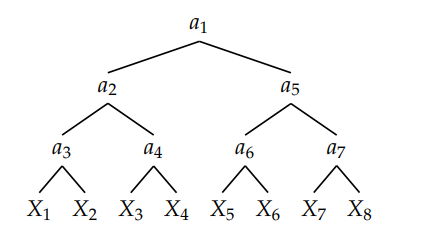
\includegraphics[width=0.5\linewidth]{image.png}
%     \label{fig:labeled}
%     \caption{Leaf $X_5$ is well-labelled if and only if \ldots}
% \end{figure}

\begin{remark}
\label{remark:LdimVSVCdim}
Littlestone dimension is a weaker notion of dimension than VC dimension. We offer three complementary perspectives:
\begin{outline}
\contribution{3 --- Original explanation with connection to model theory.}
    \1 For a leaf $v$ in a binary tree, define $P(v)$ as the set of nodes on the path from the root to $v$, where $P_L(v)$ and $P_R(v)$ represent left and right turns, respectively. A concept class $\C$ shatters a tree if, for each leaf $v$, there exists $f\in\C$ such that $f^{-1}(1)\cap P(v) = P_L(v)$. This definition is weaker than its VC analog because it requires $f$ to cut out $P_L(v)$ from $P(v)$ and not from the entire input space $X$. In essence, we restrict the input space $X$ to $P(v)$ for each leaf $v$, and make no requirements about how concepts should behave on nodes outside of these root-to-leaf paths.
    \1 The Littlestone dimension becomes equivalent to the VC dimension if we require that internal nodes at the same level have $x\in X$. This shows that the VC dimension serves as a lower bound on the Littlestone dimension, a statement we will prove later in \cref{lemma:LdimboundsVC}.
    \1 As shown in the previous section, all concept classes with finite VC dimension correspond to NIP formulas. This section will establish that finite Littlestone dimension is equivalent to a formula being stable. This connection will not surprise readers familiar with stability theory, as stable theories are a subclass of NIP theories.
\end{outline}
\end{remark}

\begin{definition}[Thicket shatter function]
\label{def:thicketfunc}
    \marginnote[0cm]{We count the maximum number of leaves labeled correctly.}
    Define the \emph{thicket shatter function} $\Lshatterfunc(m):\N\ra\N$ as 
    $$\Lshatterfunc(m):= \max \{ |L| : L\subseteq T, \C \text{ shatters } B_m \}.$$
\end{definition}

The Sauer-Shelah lemma \labelcref{lemma:Sauer-Shelah}  also holds verbatim for the thicket shatter function $\Lshatterfunc(m)$.

\begin{lemma}[Sauer-Shelah lemma, 1972]
    \label{lemma:Sauer-Shelah II}
    \contribution{0.}
    Let $\Phi_n(m):=\sum^n_{i=0}\binom{m}{i}$. If $\C$ has Littlestone dimension $n$ and $m>n$, then $\Lshatterfunc(m) \leq \Phi_n(m)$ and, in particular, $\rho_\C(m)\in O(m^n)$.
\end{lemma}
\begin{proof}
    The proof is lengthy and inductive, offering limited insight, so we omit it and refer the reader to the proof of Theorem 4.2 in \cite{Bhaskar2021}. 
\end{proof}

\begin{definition}[Mistake bound]
    \contribution{1 --- Synthesized from multiple sources, independently worded.}
    Let $f\in\C$ be a target concept and $H$ a hypothesis function. We define the \emph{mistake bound} $\mis$, as the maximum number of mistakes $H$ makes predicting $f$ on the sequence $\overline{a}=\{a_0,\ldots,a_{n-1}\}$.
\end{definition}

From now on fix a concept class $\C$ with Littlestone dimension $d$.

\begin{theorem}[Lemma 1, \cite{littlestone1988learning}]
    \label{thm:LdimMistakes}
    \contribution{0.}
    The number of mistakes of any deterministic algorithm $H$ is at least $d$.
\end{theorem}

\begin{proof}
\begin{outline}
\contribution{1 --- Improved proof structure and clarity.}
\0 By \cref{def:Ldim}, $\C$ shatters a perfect mistake tree $B_d$. We will show that an adversarial environment can force any deterministic learning algorithm to make at least $d$ mistakes:
    \1 Present the instances $x_i$ to the learner in the order they appear along a path from the root to a leaf in $B_d$.
    \1 For each prediction $h(x_i)$ made by the learner, assign the opposite truth value $1-h(x_i)$ to the instance.
\0 This strategy ensures that the learner makes a mistake on every prediction and there always exists a hypothesis $f \in \C$ consistent with all the assigned labels, due to the tree being shattered. 
Since the height of the tree is $d$, the adversary can force the learner to make at least $d$ mistakes before reaching a leaf. This holds true regardless of the specific algorithm used by the learner, as long as it is deterministic. Therefore, the number of mistakes of any deterministic algorithm on the concept class $\C$ is at least $d$, which is the Littlestone dimension of $\C$.
\end{outline}
\end{proof}

\begin{theorem}[Algorithm 2 and Theorem 3, \cite{littlestone1988learning}]
    \label{thm:SOA}
    \contribution{1.}
    \item There exists an algorithm $H$ that makes at most $d$ mistakes. The algorithm $\H$ is usually refered to as the Standard Optimal Algorithm (SOA).
\end{theorem}

\begin{proof}
\begin{outline}
\contribution{2 --- Significantly reworked original material.}
\0 We provide a constructive proof by describing the Standard Optimal Algorithm (SOA) and demonstrating its optimality.
    \1 \textbf{The algorithm:} The algorithm proceeds in rounds, maintaining a hypothesis class $V_i$ in each round $i$.
        \2 Initialization: Set $V_0= \C$.
        \2 For each round $i$:
            \3 Receive $x_i\in X$.
            \3 Partition $V_i$ into two subclasses:
            $$V_i^0:=\{f\in V_i : f(x_i)=0\} \text{ and } V_i^1:=\{f\in V_i : f(x_i)=1\},$$
            $$V_i = V_i^0 \cup V_i^1$$
\marginnote[0cm]{From a computational perspective, the computation of both VC dimension and Littlestone dimension is NP-hard. Furthermore, there is no polynomial-time algorithm that can approximate either of these dimensions to within a factor of $o(\log n)$, see \href{https://arxiv.org/abs/2211.01443}{arXiv:2211.01443}.}
            \3 Choose prediction $p_i = \argmax_{j\in\{0,1\}} \Ldim{V_i^j}$.
            \3 Receive true label $y_i$. 
            \3 Update $V_{i+1} = V_i^{y_i}$. 
    \1[] It should be noted that if $\Ldim{V_i^0} \neq \Ldim{V_i^1}$, then $y_i = 1-p_i$ unless the environment is adversarial and maximizing mistakes, hence the use of \enquote{at most} in the theorem statement.
    \1 \textbf{The optimality:} We prove that the Littlestone dimension of $V_i$ strictly decreases in each round, implying that the algorithm makes at most $d$ mistakes. Proof by contradiction:
        \2 Assume $\Ldim{V_{i+1}} \geq \Ldim{V_i}$ for some $i$. Then by construction, $V_{i+1}$ is either $V_i^0$ or $V_i^1$.
        \2 Since we choose the subclass with greater Littlestone dimension, both $\Ldim{V_i^0}$ and $\Ldim{V_i^1}$ are greater than or equal to $\Ldim{V_i}$. However, $V_i$ is the union of $V_i^0$ and $V_i^1$, which leads to the following inequality:
        $$\Ldim{V_i} \geq \min \{\Ldim{V_i^0}, \Ldim{V_i^1}\} + 1 > \Ldim{V_i},$$
        This inequality holds because $V_i$ is a mistake tree that is one level deeper than the smaller of the mistake trees $V_i^0$ and $V_i^1$. This contradiction proves our claim.
    \1[] Since the Littlestone dimension strictly decreases in each round and is initially $d$, the algorithm makes at most $d$ mistakes.
\end{outline}
\end{proof}

\begin{lemma}[Theorem 4, \cite{littlestone1988learning}]
    \label{lemma:LdimboundsVC}
    The Littlestone dimension of a concept class $\C$ is always greater than or equal to its VC dimension.
    \marginnote[0cm]{The equivalent model-theoretic statement is: \enquote{If $\phi$ is stable, then $\phi$ is NIP.}}
\end{lemma}
\begin{proof}
    Let $d$ be the VC dimension of $\C$. By definition, there exists a set $A=\{a_0,\ldots,a_{n-1}\}$ of size $d$ shattered by $\C$. Construct a perfect binary tree of height $d$ as follows: We use the elements $a_i \in A$ as labels for the internal nodes of the tree. All nodes at depth $i$ are labeled with $a_i\in A$. The leaves of this tree, which are at depth $d$, are then labeled with functions from $\C|_A$. 
    The resulting tree is shattered by $\C$ and has height $d$. This implies that the Littlestone dimension of $\C$ is at least $d$.
\end{proof}

The lemma we proved demonstrates that the gap between the Littlestone dimension and the VC dimension of a concept class $\C$ is always non-negative. Moreover, it can be arbitrarily large, as the following example illustrates.

\begin{example}
\begin{outline}
\contribution{1.}
    \0 Let $X=[0,1]$ and $\C$ the class of threshold functions on $X$. The VC dimension of $\C$ is $2$ and the Littlestone dimension is $\infty$. 
    
    \0 To demonstrate that $\C$ has infinite Littlestone dimension, we can construct an infinitely deep binary tree as follows:
        \1 Consider leaves $v_1 = \frac{1}{2}, v_2=\frac{1}{4}, v_3=\frac{1}{8},\ldots,v_i=\frac{1}{2^i}$ 
        \1 Label each leaf with 
        $$
        h_i(x)=
        \begin{cases}
            1,& x \geq \frac{1}{2^i} \\
            0,& x < \frac{1}{2^i}
        \end{cases}
        $$
    \0 For the internal nodes, we can always find values in $[0,1]$ that are consistent with the labeling of the leaves. This is possible due to the density of real numbers.
\end{outline}
\end{example}

\subsection{Stable theories}

The next section is based on Chapter 5 from \cite{Bhaskar2021}.

% We feel compelled to first describe what stable theories are about, particularly for computer scientists without a model-theoretic background. In machine learning, we are tasked with finding patterns in large datasets to make the best predictions possible. We develop models to capture these patterns, seeking a balance between simplicity and expressiveness.

% Stability theory tackles similar questions but in a more abstract, foundational setting. Developed by Saharon Shelah in the late 1960s, stability theory provides a framework to systematically classify first-order theories based on how "well-behaved" they are. At its core, stability theory is concerned with understanding the complexity of all possible configurations or "types" that can arise in a given mathematical structure.

% A stable theory, roughly speaking, is one where the number of possible types (or configurations) grows in a controlled manner as we increase the size of our domain. This is analogous to a learning problem where the number of meaningfully distinct hypotheses doesn't explode as we add more data.

% On the other hand, unstable theories exhibit a kind of \enquote{chaos}, where the number of types grows very rapidly, making classification and analysis much more difficult. In machine learning, this might correspond to situations where the complexity of potential models grows so quickly that learning becomes intractable.

% Stability theory identifies the main lines isolating stable and unstable theories and gives us tools to identify theories which are, in a sense, "mathematically learnable." In the following section, we will establish an equivalence between concept classes with finite Littlestone dimension and stable formulas. This connection will hopefully provide a different perspective on fundamental questions about structure, complexity, and learnability.

\subsubsection{Littlestone dimension and Shelah 2-rank}

\begin{remark}[Set systems and learning problems, revised]
\begin{outline}
\contribution{1.}
\0 The fundamental objects in this section are set systems.
    \1 A set system $(X,\cF, \in)$ is a structure with universe $M=X\cup \cF$, sorts $M_X$ and $M_\cF$ and equipped with a binary relation symbol $\in\subseteq M_X\times M_\cF$. For brevity, we will write $(X,\cF)$, suppresing $\in$.
    %     \1 A set system $(X,\cF, \in)$ is a two-sorted structure with universe $M=X\cup \cF$, corresponding to sorts $M^X$ and $M^\cF$, equipped with a binary relation symbol $\in\subseteq M^X\times M^\cF$. For brevity, we will write $(X,\cF)$, suppresing $\in$.
    \1 Any such set system corresponds to a learning problem $(X,\C)$, where $X$ is the input space, $\C=\{\mathds{1}_A (x) : A \in\cF\}$ is the concept class. Each concept or hypothesis function is in correspondence with a set $A\in \cF$.
\end{outline}
\end{remark}

\begin{remark}[Model-theoretic setup]
\contribution{1.}
We discuss model-theoretic assumptions and preparations we need to make in order to prove the results. We use \texttt{typewriter} script to distinguish syntactic variables $\tx, \ty$ from values $x, y$. 
\begin{outline}
    % \1 Given a partitioned first-order formula $\phi(x;y)$ and for any model $\cM$ of a complete theory $T$, define a set system $(M^\tx,M^\ty,\in)$, by $a\in b \iff \cM \models \phi(a;b)$. 
    \1 In this section, we fix a partitioned first-order formula $\phi(\tx;\ty)$ and the induced set system $(X,\cF)$ with $\cF = \{\phi(M_\tx,b) : b \in M_\ty\}$. The relation $\in$ in our set system is interpreted as $a\in F \iff \cM\models\phi(a;b)$ for the $b$ that defines $F$. 
    \1 We fix a sufficiently saturated model $\cM$ of the theory $\Th(X,\cF)$ to ensure that all types are realized, which may affect later rank calculations if, for example, we work in a model which doesn't realize many types. Whenever we assert that some sentence holds, we always mean relative to the model $\cM$.
    % \1 In this context, we focus on concept classes generated by a single fixed formula $\phi(x;F)$. This approach allows us to study a wide range of geometrically interesting concept classes, for example
    %     \2 circles in $\R^2$, given by $\phi(x;y) := (x_1-y_1)^2 + (x_2-y_2)^2 < y_3^2$,
    %     \2 half-spaces in $\R^n$, given by $\phi(x;w,b)) = \sum w_i \cdot x_i + b \geq 0$,
    %     \2 polynomials in $\R^2$ of degree at most $d$, given by $\phi(x;y)=\sum_{i=0}^d y_i x_1^i = x_2$,
    %     \2 elliptic curves in $\bC$, given by $\phi(x,y;a,b)=y^2=x^3+ax+b$.
\end{outline}
\end{remark}

In our previous discussion (\cref{remark:consistentRealizable}), we focused on consistent and realizable cases. To extend this concept into model-theoretic terms, we will now introduce the notion of partial $\phi$-types.

\begin{definition}
\begin{outline}
\contribution{1.}
\0 Let $\phi$ be the formula $\tx\in \tF$. We define:
    \1 A \emph{$\phi$-formula} is either $\phi(x;\tF)$ or $\lnot\phi(x;\tF)$ for some $x\in M_x$. For brevity, we denote $\phi(x;\tF)^1=\phi(x;\tF)$ and $\phi(x;\tF)^0 = \lnot \phi(x;\tF)$.
    \1 A \emph{finite $\phi$-type} $p$ is a conjunction of $\phi$-formulas, including the \emph{empty conjunction} $\top$. We denote by $p(\cF)$ the subfamily of $\cF$ satisfying the type $p$.
    \1 Two finite $\phi$-types $p$ and $q$ are \emph{contradictory}, if there exists $x\in X$ and $t\in\{0,1\}$ such that:
        \2 $\phi(x;\tF)^t\in p$,
        \2 $\phi(x;\tF)^{1-t}\in q$
    \1[] In this case, we say $p$ and $q$ disagree on $\phi(x;\tF)$.
\end{outline}
\end{definition}

How does the notion of a partial $\phi$-type relate to online learning? As we receive observed data in the form of pairs $(x_i, y_i)$, where $x_i \in X$ represents an instance and $y_i \in {0,1}$ represents its label, we can enforce consistency in our structure $(X, \cF)$ by requiring either $\phi(x_i;\tF)$ or $\lnot\phi(x_i;\tF)$ to hold in $(X, \cF)$, depending on the value of $y_i$. 
This process effectively restricts our concept class to only those concepts that agree with the observed data and the collection of these restrictions is what we now defined as a finite $\phi$-type. The subfamily of $\cF$ that satisfies these constraints is written as $p(\cF)$. This represents the set of concepts in our class that are consistent with the observed data so far.

Now, we formalize \cref{def:labeling} describing conditions under which a tree $T$ admits $(X,\cF)$ consistent with a finite $\phi$-type $p$. 

\begin{definition}[Definition 5.1, \cite{Bhaskar2021}]
\label{def:adm}
\contribution{1 --- Improved structure and clarity.}
Let $T$ be an unordered tree with non-leaves $N$ and leaves $L$. We define 
    \begin{outline}
        \1 a signature $\cL_T = \{\in\} \cup \{a_u : u\in N\} \cup \{b_v : v\in L\}$, where 
            \2 $\in$ is a binary relation symbol $\subseteq X \times \cF$
            \2 ${a_u : u \in N}$ are constant symbols of sort $X$
            \2 ${b_v : v \in L}$ are constant symbols of sort $\cF$
        \1 a first-order $\cL_T$-theory $\Adm{T}{p}$ with the following axioms:
            \marginnote[0cm]{For simplicity, we will occasionally denote the constants $a_u$ or $b_v$ as the image $\alpha(u)$ or $\alpha(v)$ of the respective node under a valid labeling $\alpha$.}
            \2[(1)] $p(b_v)$ for any $v\in L$,
            \2[(2)] $\phi(a_u;b_v)\not\leftrightarrow \phi(a_u;b_w)$ if $v\bot_u w$,
            \2[(3)] $\phi(a_u;b_v)\leftrightarrow \phi(a_u;b_w)$ if $v\sim_u w$.
    \end{outline}
\end{definition}

If $(X,p(\cF))$ admits $T$, then $\Th(X,p(\cF))\cup \Adm{T}{p}$ is consistent. This means there exists a model which simultaneously satisfies both $\Th(X,\cF)$ and $\Adm{T}{p}$.
Since $\cM$ is sufficiently saturated, the consistency of $\Th(X,\cF)\cup \Adm{T}{p}$ is equivalent to the admissibility of $T$ in $\cM=(M_X, p(M_\cF))$.

\begin{example}
\label{example:Discussion}
\begin{outline}
\contribution{3 --- This is original.}
    \0 Let $X=\{1,2,3,4\}$ and $\cF = \{\{1,2\},\{3,4\},\{1,3\}\}$. We consider the structure $(X,\cF)$ with the signature $\cL = \{\in\}$. 
    The theory of $(X,\cF)$ is the set of all first-order $L$-sentences true in $(X,\cF)$. For example, the sentence \enquote{there are exactly 3 sets in $\cF$} can be expressed as:
    $$\exists x_1,x_2,x_3:
    \left(\bigwedge_{i=1}^3 x_i \in M_\cF\right) 
    \land 
    \left(\bigwedge_{i=1}^2 x_i\neq x_{i+1}\right)
    \land 
    \left(\forall y: y\in M_\cF \land \bigvee_{i=1}^3 y=x_i\right).
    \footnote{Here $x\in M_\cF$ means \enquote{$x$ is of sort $M_\cF$}.}$$
    
    Define a partial $\phi$-type $p(\tF) = \{\lnot\phi(4;\tF)\}$. 
    This implies $p(\cF)=\{\{1,2\},\{1,3\}\}$.
    
    Now consider a tree $T$ with one root $u$ and two leaves $v,w$. We expand the signature to $\cL_T=\{\in, a_u,b_v,b_w\}$, where $a_u$ is a constant symbol of sort $X$ and $b_v,b_w$ are constant symbols of sort $\cF$. 
    The theory $\Adm{T}{p}$ consists of the following $\cL_T$-sentences:
    $$\{4\not\in b_v, 4\not\in b_w, a_u\in b_v
    \not\leftrightarrow a_u\in b_w\}.$$
    We will now verify the equivalence between the consistency of $\Th(X,\cF)\cup \Adm{T}{p}$ and $T$ admitting $(X,\cF)$:

        \1[$\impliedby$:] If $T$ admits $(X,p(\cF))$, then there exists a valid labeling $\alpha$. In our example, $\alpha$ is given by $\alpha(u)=3, \alpha(v)=\{1,3\}, \alpha(w)=\{1,2\}$. 
            \2 The property (1) holds by construction, since $4\not\in\{1,3\}$ and $4\not\in\{1,2\}$ is both in $\Th(X,\cF)$ and $\Adm{T}{p}$.
            \2 The properties (2) and (3) hold since $3\in \{1,3\}$ and $3\not\in \{1,2\}$, so $\Th(X,\cF)$ and $\Adm{T}{p}$ are consistent.
        \1[$\implies$:] If $\Th(X,\cF)\cup \Adm{T}{p}$ is consistent, then there exists an interpretation in $\cM$ of the constants $a_u, b_v, b_w$ that satisfies property $(1),(2),(3)$. This interpretation provides a valid labeling $\alpha$ of $T$. 
            \2 This equivalence doesn't necessarily hold for infinite trees. To see why, suppose $\Th(X,\mathcal{F}) \cup \Adm{T}{p}$ is consistent. By the Löwenheim-Skolem theorem, it has a countable model $(X',\cF')$. Since $T$ is infinite, it has $2^\omega$ leaves. For $T$ to be admissible in $(X',\cF')$, we would need an injective map from the leaves $L$ to $F'$. This is equivalent to having an injection from $2^\omega$ to $\omega$, wihch is impossible.
    \0 The moral of the story is that, at least in the finite case, the consistency of $\Th(X,\cF)\cup \Adm{T}{p}$ hinges on the existence of a valid labeling $\alpha: T\rightarrow X\cup p(\cF)$. This labeling exists only in a sufficiently saturated model where every leaf type is realized.
\end{outline}
\end{example}

In essence, $\Adm{T}{p}$ is a formal way of saying that $T$ can be properly labelled by elements of $X$ and $\cF$ that satisfy $p$, in a way that respects the branching structure of $T$. This is probably one of the reasons why \cite{hodges} describes Shelah $2$-rank as the branching index. 

\begin{example}
\contribution{3.}
    Imagine you are a network engineer working for a large university campus. The IT department wants to optimize WiFi coverage across the campus grounds. They need to understand the actual coverage area of each WiFi access point, which is theoretically circular and has uniform signal strength. At point $(x,y)=(1,1)$ there is signal and at point $(x,y)=(3,3)$ there is no signal. Then we can translate the concepts in online learning and model theory as in \cref{tab:translation}.
    \begin{table}[h]
    \centering
        \begin{tabular}{p{0.45\textwidth}|p{0.45\textwidth}}
        \textbf{Online learning} & \textbf{Model theory} \\
        \hline
        Input space: 2D real plane & $X = \mathbb{R}^2$ \\
        Concept: Interior of a circle with center $(y_1,y_2)$ and radius $y_3$ & $\phi(x_1,x_2;y_1,y_2,y_3) := (x_1-y_1)^2 + (x_2-y_2)^2 < y_3^2$ \\
        Hypothesis class: Circles in $\mathbb{R}^2$ & $\cF = \{\mathds{1}_{\phi(M_x;b)} : b \in \R^3\}$ \\
        Labeled examples: $(1,1)$ is positive, $(3,3)$ is negative & $p(\tF) = \{\phi(1,1;\tF), \neg\phi(3,3;\tF)\}$ \\
        Hypothesis class consistent with observed data & $(X, p(\mathcal{F}))$ \\
        Mistake tree $T$ & $T$ \\
        Conditions for a mistake tree $T$ to admit $\C$ & $\text{Adm}_p^T$ \\
        Littlestone dimension & Shelah 2-rank
        \end{tabular}
    \caption{Dictionary of terms between online learning and model theory}
    \label{tab:translation}
    \end{table}
\end{example}

Now we are ready to define a local version of Morley rank, the Shelah 2-rank.

\begin{definition}[Shelah 2-rank]
\label{def:shelah2rank}
\begin{outline}
\contribution{1.}
%\marginnote[0cm]{We use a slightly simplified version of the Shelah 2-rank. Usually it is defined for $p$ over some set of formulas $\Delta$, here $\Delta = \{\phi\}$.}
\0 For any finite $\phi$-type $p(\tF)$, define the \emph{Shelah 2-rank} $\shelahrank$ 
    \1[1)] $\shelahrank \geq 0$ if $p$ is consistent, i.e. there exists some $b\in M_\cF$ such that $p(b)$ holds.
    \1[2)] For any finite $k$, $\shelahrank \geq k + 1$ if there exists a pairwise contradictory family of types $\{p_i : i<\omega\}$ such that $\shelah{p_i} \geq k$ for all $i<\omega$.
    \marginnote[0cm]{Some definitions require only two contradicting types. The definitions are equivalent and we will implicitly prove this later.}
    \1[3)] $\shelahrank=\infty$ if $\shelahrank\geq k$ for all $k < \omega$.
    \1[4)] $\shelahrank = -\infty$ if $p$ is inconsistent.
\end{outline}
%\marginnote[0cm]{This requirement trivially excludes finite $\cF$ since finitely many functions cant realize infinite number of different types. Finite $X$ is okay.}
\end{definition}
% Note that this excludes finite $\cF$ since the chain becomes stationary after some N. This is fine, because this means that \cF has finite variation so its rank is 0. <= Corollary or Lemma

The second condition in \cref{def:shelah2rank} allows us to infer the existence of an additional order structure on types $\{p_i : i<\omega\}$, which can be extracted as an infinite sequence.

\begin{lemma}[Lemma 5.6, \cite{Bhaskar2021}]
\label{lem:infSet}
\contribution{0.}
    Suppose $\{p_i : i<\omega\}$ is a sequence of pairwise contradictory finite $\phi$-types. Then there exists an infinite set $S\subseteq \omega$ such that for any $r\in S$, there exists $a\in M_X$, such that for any $s>r$ in $S$, $p_r$ and $p_s$ disagree on $\phi(a,\tF)$.
\end{lemma}
\begin{proof}
    \begin{outline}
    \contribution{1 --- Improved proof structure and clarity.}
    \0 We will construct $S$ inductively as follows: 
        \1 Let $S_0 = \omega$.
        \1 For any $S_i\subseteq \omega$ let $m_i$ be its least element. 
            \2 Consider finite $\phi$-type $p_{m_i}$ consisting of finitely many formulas $\{\phi(x_i;\tF)^t : i<\omega, t\in 2\}$. 
            \2 Since any two types are pairwise contradictory, there exists set $S_{i+1}\subseteq S_i\setminus \{m_i\}$ such that $\phi(x_i;\tF)^t$ occurs in $p$ and $\phi(x_i;\tF)^{1-t}$ occurs in infinitely many $(p_j)_{j\in S_{i+1}}$. 
        \1 This construction gives us 
            \2 A descending chain of index sets $S_0 \supset S_1 \supset S_2 \supset \ldots$, 
            \2 An increasing sequence of indices $m_0 < m_1 < m_2 < \ldots$,
            \2 A sequence of elements $x_0,x_1,x_2,\ldots$ 
        \1[] such that 
            \2 For all $j>i$, $p_{m_j}$ and $p_{m_i}$ disagree (uniformly) on $\phi(x_i,\tF)$,
            \2 For each $k<i$, $p_{m_k}$ and $p_{m_i}$ disagree (non-uniformly) on $\phi(x_k,\tF)$.
    \0 Therefore $S=\{m_0,m_1,\ldots\}$ has precisely the qualities we seek.
    \end{outline}
\end{proof}

The rank of $p(\cF)$ is determined by two key factors: its consistency and its ability to be split into disjoint sets. If $p(\cF)$ is non-empty, meaning there exists some $F\in\cF$ that realizes $p$, its rank is $0$. This corresponds to restricting the concept class $\C$ to functions that are consistent with the observed data. 
The rank is $1$ if there exists some $a\in M_X$ such that both $p\land \phi(a;\tF)^0$ and $\phi(a;\tF)^1$ are consistent. In this case, we can split $p(\cF)$ into two disjoint sets that disagree on $\phi(a;\tF)$. This splitting behavior is analogous to the mistake trees discussed in the previous section. 

The ability to continue this branching process determines the number of distinct types that $\phi$ can exhibit. Each split potentially doubles the number of types, corresponding to the different ways of extending $p$ consistently. In fact, this branching behavior is what ultimately determines the number of types $\phi$ exhibits. It is this limitation on infinite branching that characterizes stable theories as \enquote{tame}, distinguishing them from theories where such branching can proceed without bound.

\begin{center}
\begin{figure}
\centering
\begin{tikzpicture} % an infinite 2-branching tree
\Tree
[ 
	[ 
		[ .$\circ$
		]
		[
			[ .$\circ$
			]
			[ 
				[ .$\circ$
				]
				[ .$\vdots$
				]
			]
		]
	] \edge[thick];
	[ 
		[ 
			[ .$\circ$
			]
			[
				[ .$\circ$
				]
				[ 
					[ .$\circ$
					]
					[ .$\vdots$
					]
				]
			]
		] \edge[thick];
		[
			[ 
				[ .$\circ$
				]
				[
					[ .$\circ$
					]
					[ 
						[ .$\circ$
						]
						[ .$\vdots$
						]
					]
				]
			] \edge[thick];
			[ 
				[ 
					[ .$\circ$
					]
					[
						[ .$\circ$
						]
						[ 
							[ .$\circ$
							]
							[ .$\vdots$
							]
						]
					] 
				] \edge[thick];		
				[ .$\vdots$
				]
			]
		]
	]
]

\end{tikzpicture}
\caption{The infinite 2-branching tree. The \emph{spine }is indicated by the
thick edge. The vertices of any $T_{k+1}$ can be partitioned into
the vertices on the spine, plus countably many copies of $T_{k}$.}
\end{figure}
\end{center}

\begin{definition}[$k$-branching trees]
    \label{def:kTree}
    \contribution{0.}
    Define $0$-branching tree as a single leaf. For $k\geq 1$, the $k$-branching tree $T_k$ is the unordered binary tree with subtrees $T_k$ and $T_{k-1}$. The dimension of $T_k$ is $k$. Note, that any $T_k$ contains a  perfect binary tree $B_k$.
\end{definition}

\begin{theorem}[Theorem 5.9, \cite{Bhaskar2021}]
\label{thm:ShelahAdm}
\contribution{2 --- The original proof is one page long and skips over important details. We significantly improved structure of the proof and added many new comments and explanations.}
    The following conditions are equivalent:
    \begin{outline}
        \1[1)]$\shelahrank \geq k$,
        \1[2)]$\Th(X,\cF) \cup \Adm{T_k}{p}$ is consistent.
    \end{outline}
\end{theorem}

\begin{proof}
We work in a sufficiently saturated model $\cM$ of $\Th(X,\cF)$. Since it is sufficiently saturated, the admissibility of $T_k$ in $\cM$ is equivalent to the consistency of $\Th(X,\cF)\cup \Adm{T_k}{p}$, as discussed in \cref{example:Discussion}. We use induction:
\begin{outline}
    \1 Base case: Show that the equivalence holds trivially for $k=0$.
        \2 By \cref{def:shelah2rank}, $\shelahrank \geq 0$ iff there exists some $F\in M_\cF$ which satisfies $p$, that is $\cM\models p(F)$.
        \2 By \cref{def:kTree}, $T_0$ consists of a single leaf $v$ and zero non-leaves, so the labeling $\alpha: v \mapsto F$ is valid and equivalent to the consistency of $\Th(X,\cF)\cup \Adm{T_0}{p}$ by the discussion in \cref{example:Discussion}.
\0 Now comes the inductive step, where we assume the equivalence holds for $k$ and prove it for $k+1$.
    \1 Assume $\shelahrank\geq k+1$:
        \2 By \cref{def:shelah2rank}, there exists a family of pairwise contradictory types $\{p_i : i<\omega\}$ witnessing $\shelahrank \geq k+1$.
        \2 By \cref{lem:infSet} there exists an infinite set $S\subseteq\omega$ such that $\{p_i : i\in S\}$ also witnesses $\shelahrank \geq k+1$, with the following additional property:
        $$\forall r \in S : \exists a(r) \in M_X : \forall s > r : p_r \text{ and } 
        p_s \text { disagree on } a(r).$$
        We can assume without loss of generality that our original family already has this property. This is because we can relabel the types $p_i$ using only indices from $S$ and discard the unwanted types, resulting in a subfamily that still witnesses $\shelahrank\geq k+1$ and has this additional structure.
        \2 Consider the infinite $k+1$-branching tree $T_{k+1}$. It can be visualized as consisting of a single infinite spine with countably many copies of $T_k$ branching off from it. We partition the nodes of $T_{k+1}$ as follows:
            \3 The set of non-leaves $N$ is partitioned as 
            $$N=\left(\bigcup_{i<\omega} N_i \right) \cup N_s,$$
            where $N_i$ is the set of non-leaves in the $i$-th copy of $T_k$ and $N_s$ is the set of vertices along the spine. 
            \3 The set of leaves $L$ is partitioned as 
            $$L=\bigcup_{i<\omega} L_i,$$
            where $L_i$ is the set of leaves in the $i$-th copy of $T_k$.
        \2 By assumption, we have $\shelah{p_{i}}\geq k$ for each $i<\omega$. Therefore by inductive hypothesis, $\Th(X,\cF)\cup\Adm{T_k}{p\land p_i}$ is consistent for each $i$. This implies that each copy of $T_k$ admits a valid labeling $\alpha_i: N_i \rightarrow M_X, L_i \rightarrow M_\cF$. 
        \2 We now construct a labeling $\alpha$ of $T_{k+1}$ by combining all valid labelings $\alpha_i$. Define $\alpha: N\cup L \rightarrow M_X \cup M_\cF$ as follows:
            \3 For each $i<\omega$ and $v\in N_i \cup L_i$ let $\alpha(v)=\alpha_i(v)$ 
            \3 For each $r<\omega$ and $v$ the $r$-th node on the spine $N_s$ let $\alpha(v)=a(r)$
        \2 We will now verify that $\alpha$ is a valid labeling by checking axioms (1), (2), and (3) from \cref{def:adm}:
            \3 For any leaf $v\in L$, $\alpha(v)$ satisfies $p\land p_i$ for some $i$, which implies $\alpha(v)$ satisfies $p$,
            \3 For any two leaves $v,w\in L$ and their common ancestor $u\in N$ there are four possible combinations:
% \marginnote[0cm]{Explained in plain language, we observe four possible situations:
\marginnote[0cm]{
\begin{tikzpicture}[remember picture,overlay]
    \node[anchor=west] at (0,0) {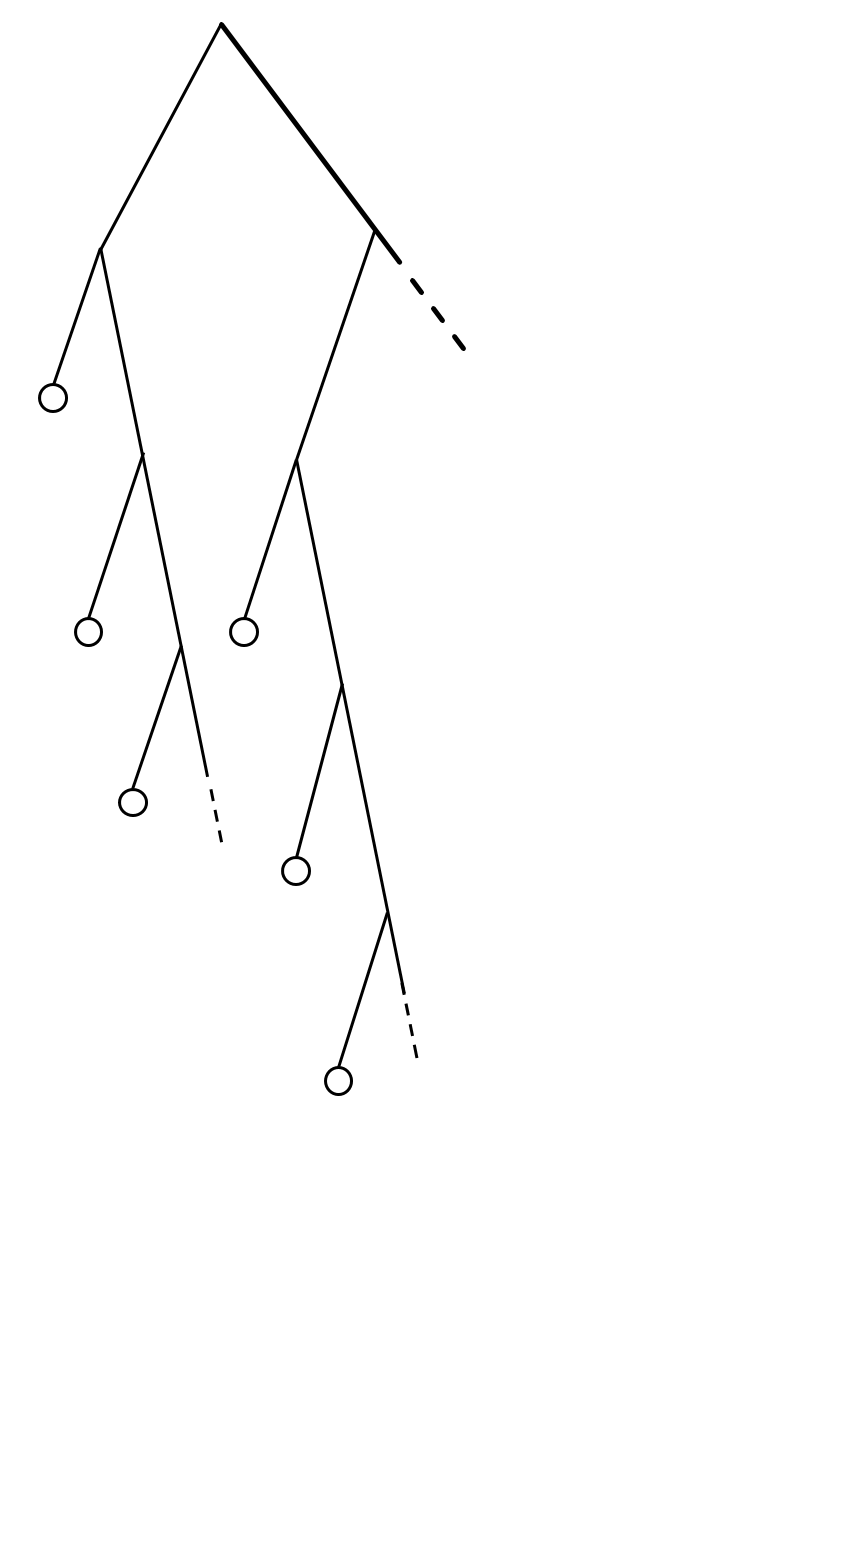
\includegraphics[width=\marginparwidth]{marginTree2.png}};
    \node[anchor=center] at (0.39,2.5) {$u$};
    \node[anchor=center] at (0.34,1.45) {$v$};
    \node[anchor=center] at (0.51,0.40) {$w$};
\end{tikzpicture}}
                \4 If $v,w\in L_i$ and $u\in N_i$ for some $i$, the conditions are inherited from $\alpha_i$.
                \4 If $v,w\in L_i$ and $u\in N_s$, then $v$ and $w$ always will be in the same subtree relative to $u$ and $u$ must be the $r$-th node on the spine, $r \leq i$.\\
                Both $\alpha(v),\alpha(w)$ satisfy the type $p\land p_i$. By properties, established in \cref{lem:infSet}, all realizations of $p_i$ agree on all previous nodes $a(r)$ for all $r\leq i$. Therefore, $$\phi(a(r);\alpha(v))\leftrightarrow\phi(a(r);\alpha(w)).$$
\marginnote[0cm]{
\begin{tikzpicture}[remember picture,overlay]
    \node[anchor=west] at (0,0) {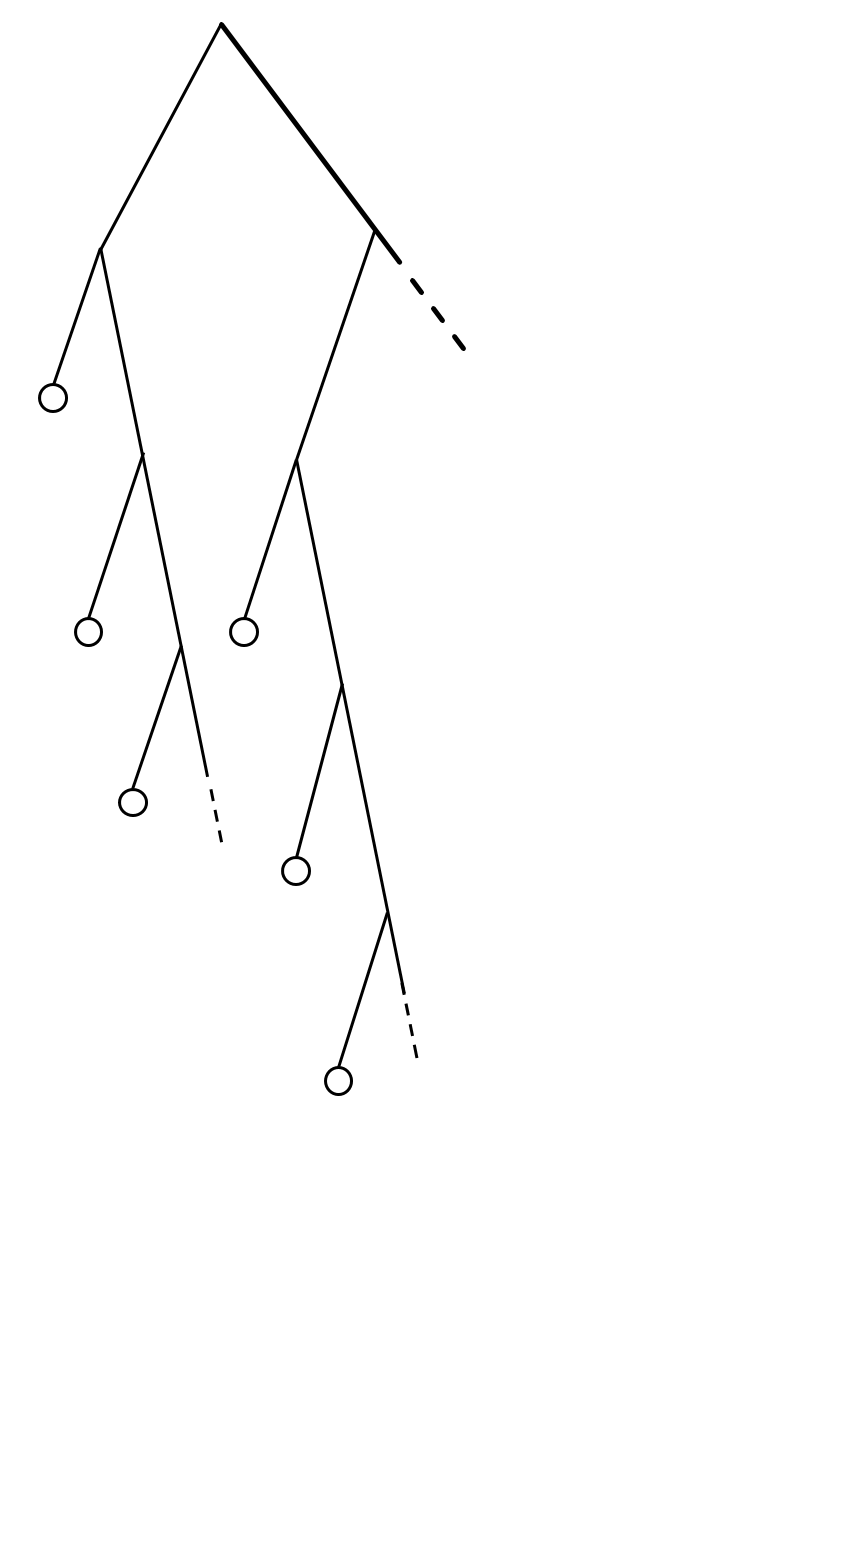
\includegraphics[width=\marginparwidth]{marginTree2.png}};
    \node[anchor=center] at (2,2.7) {$u$};
    \node[anchor=center] at (1.3,0.35) {$v$};
    \node[anchor=center] at (1.5,-0.8) {$w$};
\end{tikzpicture}}
                % If I expand Lemma 3.3 or even make a new lemma stating properties explicitly, I can cut back here and add before that.
% \marginnote[0cm]{$v,w$ in different $T_k$ and $u$ on the spine, but before $v$ branch.} 
                \4 If $v\in L_i$ and $w\in L_j$ for $i<j$ and $v$ and $w$ are in the same subtree relative to $u$.\\
                Then $u$ must be the $r$-th node on the spine and $r<i$. By properties established in \cref{lem:infSet}, $\alpha(v)$ and $\alpha(w)$ agree on all previous nodes $a(r)$ for all $r < i$. Therefore 
                $$\phi(a(r);\alpha(v))\leftrightarrow\phi(a(r);\alpha(w)).$$
\marginnote[0cm]{\begin{tikzpicture}[remember picture,overlay]
    \node[anchor=west] at (0,0) {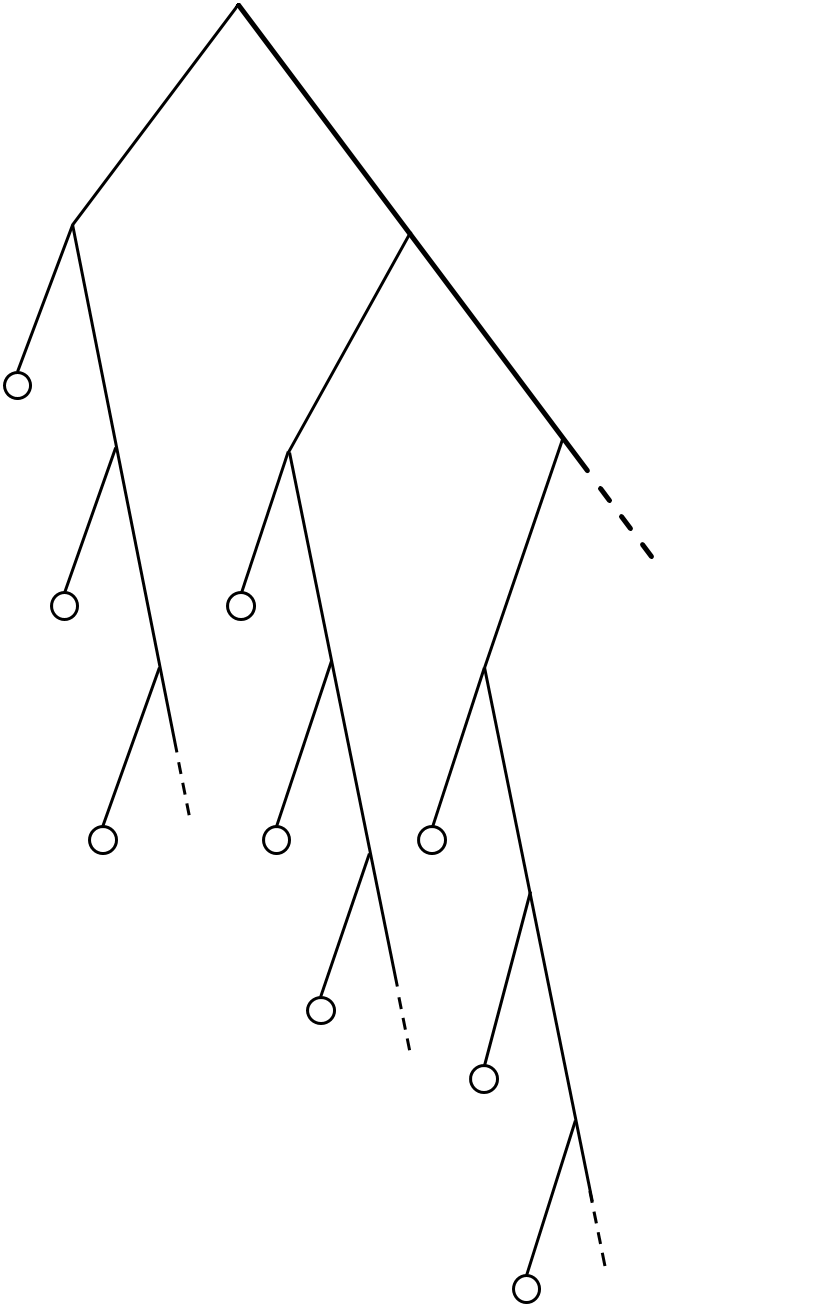
\includegraphics[width=\marginparwidth]{marginTree3.png}};
    \node[anchor=center] at (1.2,3.4) {$u$};
    \node[anchor=center] at (1.6,-2.1) {$v$};
    \node[anchor=center] at (2.45,-2.4) {$w$};
\end{tikzpicture}}
% \marginnote[0cm]{$v,w$ in different $T_k$ and $u$ on the spine, but right where $v$ branch starts.}
                \4 If $v\in L_i$ and $w\in L_j$ for $i<j$ and $v$ and $w$ are in different subtrees relative to $u$.\\
                Then $u$ is the $r$-th node on the spine and $r=i$. Yet again, by properties established in \cref{lem:infSet}, $\alpha(v)$ and $\alpha(w)$ disagree on $a(i)$, therefore
                $$\phi(a(i);\alpha(v))\not\leftrightarrow\phi(a(i);\alpha(w)).$$
        \2 We have now proven that $\alpha$ is a valid labeling of $T_{k+1}$ and since $\cM$ is sufficiently saturated it is equivalent to $\Th(X,\cF) \cup \Adm{T_{k+1}}{p}$ being consistent. This concludes the forward direction.
    \1 Assume $\Th(X,\cF)\cup \Adm{T_{k+1}}{p}$ is consistent in $\cM$.
        \2 By discussion in \cref{example:Discussion}, $(X,p(\cF))$ admits $T_{k+1}$. This is equivalent to the existence of a valid labeling $\alpha: T_{k+1} \rightarrow X \cup p(\cF)$ satisfying axioms $(1),(2),(3)$ of \cref{def:adm}.
        \marginnote[0cm]{
        \begin{tikzpicture}[remember picture,overlay]
            \node[anchor=west] at (0,0) {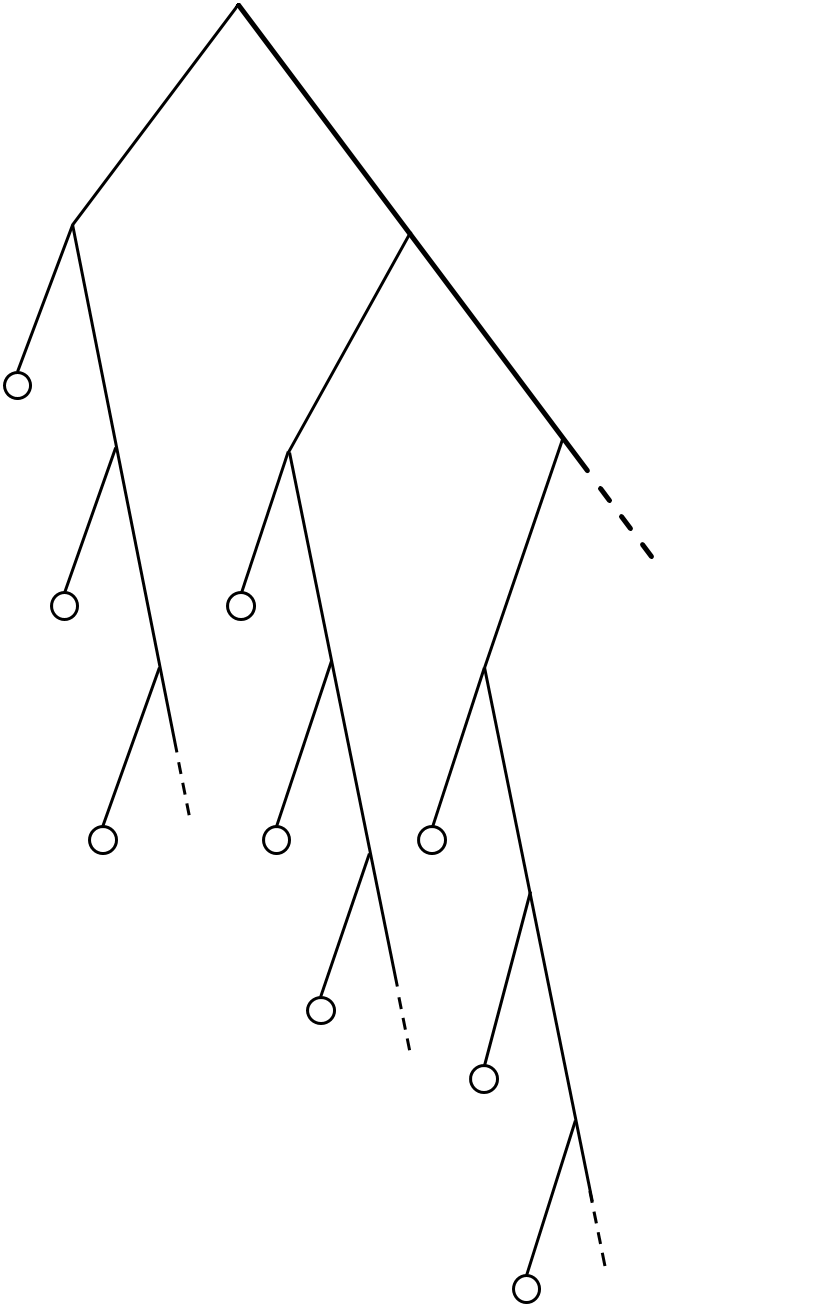
\includegraphics[width=\marginparwidth]{marginTree3.png}};
            \node[anchor=center] at (2.3,2.1) {$u$};
            \node[anchor=center] at (1.6,-2.1) {$v$};
            \node[anchor=center] at (2.45,-2.4) {$w$};
        \end{tikzpicture}}
        \2 Let $N_s, N_i, L_i$ be as discussed above and let $a(i)$ be the label of the $i$-th node along the spine. 
        \2 By axiom $(2)$, for each $i<\omega$, all leaves $v$ in $i$-th copy of $T_k$ must agree on the truth value of $\phi(a(i); \alpha(v))$, since for any two such leaves $v,w$, we have $v\sim_{a(i)}w$.  
        \2 For $i<\omega$, define 
        $$p_i = \{\phi^t(a(i),\cF)\} \cup \{\phi^{1-t}(a(i'),\cF): i' < i\},$$ 
        where $t\in\{0,1\}$ is chosen such that $\phi^t(a(i),\tF)$ is satisfied by the leaves in the $i$-th copy of $T_k$. 
        \2 For each $i<\omega$, consider the restriction $\alpha|_{T_k^i}$ of $\alpha$ to the $i$-th copy of $T_k$. This restriction inherits properties $(2)$ and $(3)$ from the original labeling $\alpha$. For property $(1)$, observe that for each $v\in L_i$, $\alpha(v)$ satisfies $p\land p_i$ by construction of $p_i$. 
        \2 By the inductive hypothesis, this implies $\shelah{p_i} \geq k$ for each $i<\omega$. Note that for each $i<j$, $p_i$ and $p_j$ disagree on $\phi(a(i); \tF)$. Thus, $\{p_i : i < \omega\}$ forms a pairwise contradictory family of types. By \cref{def:shelah2rank}, the existence of this family with $\shelah{p_i}\geq k$ implies $\shelahrank \geq k+1$. This concludes the proof of the reverse direction.
\0 Having established both directions, we have shown that $\shelahrank \geq k+1$ if and only if $\Th(X,\cF)\cup \Adm{T_{k+1}}{p}$ is consistent, completing the inductive step.
\end{outline}
\end{proof}

Our main result in this section establishes the equivalence between finite Littlestone dimension and finite Shelah 2-rank.
The original paper by Bhaskar \cite{Bhaskar2021} doesn't give a direct proof, so we will give it in full, bringing together the arguments.

To quantify the growth of the shatter function $\rho(m)$ (see \cref{def:thicketfunc}), we introduce the intermediate concept of thicket density. This density is defined as the least exponent bounding the growth rate of $\rho(m)$, serving as a crucial link between finite and infinite structures.

\begin{definition}[Definition 4.5, \cite{Bhaskar2021}]
\label{def:thicketDens}
\begin{outline}
\contribution{0.}
\0 Let $\rho(m)$ be the thicket shatter function of $(X,\cF)$, as defined in \cref{def:thicketfunc}. The \emph{thicket density} of $(X,\cF)$, denoted by $\dens(X,\cF)$, is defined as $\inf\{c\in \R : \rho(m) \in O(m^c)\}$. 

\0 If $\rho(m) \in O(m^c)$ for all $c\in\R$ then $\dens(X,\cF)=-\infty$ and if $\rho(m) \not\in O(m^c)$ for all $c\in\R$ then $\dens(X,\cF)=\infty$.
\end{outline}
\end{definition}

The key challenge lies in transitioning from the inadmissibility of the infinite tree $T_k$ to the inadmissibility of the finite tree $B_k$. While it's straightforward to show that admitting $T_k$ implies admitting $B_k$, the reverse implication requires careful analysis of asymptotic behavior. Thicket density allows us to bridge this gap effectively.

\begin{table}[h]
\centering
    \begin{tabular}{p{0.30\textwidth} p{0.30\textwidth} p{0.30\textwidth}}
    Littlestone dimension & Thicket density & Shelah 2-rank\\
    \hline
    Admissibility of finite tree $B_k$ & Rate of asymptotic growth & Admissibility of infinite tree $T_k$
    \end{tabular}
\end{table}

The main challenge arises from the fact that $T_k$ can be very deep and unbalanced, potentially having any finite number of leaves. Consequently, finding one admissible embedding of $B_k$ in $T_k$ doesn't guarantee that it will fully label $T_k$. Thicket density provides a way to overcome this obstacle by analyzing the asymptotic growth rate of admissible labelings, thereby connecting the finite structure of $B_k$ to the infinite structure of $T_k$.

The original proof goes through for thicket density, briefly mentioning at the end that in case of Littlestone dimension, density and dimension are equivalent as $\N\cup\{\infty,-\infty\}$-valued quantities. We decided to change the arguments and instead give an \enquote{honest} proof, instead bounding Littlestone dimension by thicket density and thicket density by the Shelah 2-rank.

\begin{theorem}[Theorem 4.4, \cite{Bhaskar2021}]
\label{lem:finiteTreeForbidden}
\contribution{2.}
    If $\shelahrank < k$, then $\dens(\C_\phi) < k$.
\end{theorem}
\begin{proof}
\begin{outline}
\0 Assume $\shelahrank < k$:
    \1 By \cref{thm:ShelahAdm} $\Adm{T_{k}}{p}$ is inconsistent with $\Th(X,\cF)$. By compactness theorem, there exists a finite subtree $S$ of $T_k$ such that $\Adm{S}{p}$ is inconsistent with $\Th(X,\cF)$. By discussion in \cref{example:Discussion}, $(X,p(\cF))$ forbids $S$. Since $T_k$ has dimension $k$, $S$ has dimension at most $k$. Therefore, $(X,p(\cF))$ forbids some finite tree $S$ of dimension $k$.
\0 We prove that if $(X,p(\cF))$ forbids a finite tree $S$ of dimension $k$, then $\dens(X,p(\cF))<k$. Proof by induction on construction of $T$: 
    \1 Base case: If $S$ has dimension 0, it is the single leaf $B_0$. If $(X,p(\cF))$ forbids $S$, then $p(\cF)$ must be empty, hence its Littlestone dimension is $-\infty < 0$.
    \marginnote[0cm]{$S$ of dimension $k$\\ $S_1,S_2$ of dimension $k_1,k_2 < k$}
    \1 Inductive step: Suppose $S$ has subtrees $S_1$ and $S_2$ with dimensions $k_1$ and $k_2$. By the inductive hypothesis, there exist functions $f_1(n)\in O(n^{k_1-1})$ and $f_2(n)\in O(n^{k_2-1})$ that serve as upper bounds on the thicket shatter functions $\rho_1(n)$ and $\rho_2(n)$ if they forbid $S_1$ or $S_2$ respectively.
    \marginnote[0cm]{$\rho_1 \leq f_1\in O(n^{k_1-1})$\\
    $\rho_2 \leq f_2\in O(n^{k_2-1})$\\ 
    $\rho \leq \rho_1 + \rho_2$}
        \2 For $x\in X$, let $\cFx = \{A\in\cF : x\in A\}$ and $\cFnotx = \{A\in\cF : x\not\in A\}$ with thicket shatter functions $\rhox$ and $\rhoNotx$ respectively.
            \marginnote[0cm]{$\rhox, \rhoNotx$}
            \3 Let $P_i(x)$ express that $(X,\cFx)$ admits $S_i$. 
            \3 Let $Q_i(x)$ express that $(X,\cFnotx)$ admits $S_i$. 
        \2 Then $(X,p(\cF))$ admits $S$ if and only if:
        $$\exists x\in X 
        \left(
        \left(P_1(x)\land Q_2(x)\right)
        \lor
        \left(P_2(x)\land Q_1(x)\right)
        \right)
        $$
        \2 Reasoning propositionally, $(X,p(\cF))$ forbids $S$ if and only if 
        \begin{align*}
            \forall x\in X 
            (\lnot P_1(x)\land\lnot P_2(x))
            & \lor
            (\lnot P_1(x)\land\lnot Q_1(x))
            \lor \\
            (\lnot Q_2(x)\land\lnot P_2(x))
            & \lor 
            (\lnot Q_2(x)\land\lnot Q_1(x))
        \end{align*}
        \2 By the inductive hypothesis, this implies:
        \begin{align*}
            \forall x\in X
            (\rhox\leq f_1 \land \rhox\leq f_2) 
            &\lor
            (\rhox\leq f_1 \land \rhoNotx\leq f_1)
            \lor \\
            (\rhoNotx\leq f_2 \land \rhox\leq f_2)
            &\lor
            (\rhoNotx\leq f_1 \land \rhoNotx\leq f_2),
        \end{align*}
        where $\rhox\leq f_1$ abbreviates $\forall n<\omega: \rhox(n)\leq f_1\in O(n^{k_1-1})$. Label the four cases (1)-(4) respectively.
        \2 We consider two cases. 
            \3 If (2) and (3) hold, then $\rhox \leq f_1$ and $\rhoNotx \leq f_1$, which implies $\rho \leq \rhox + \rhoNotx \leq 2f_1 \in O(n^{k-1})$.
            \3 If (1) and (4) hold, then reasoning propositionally:
            \begin{align*}
            & \forall x\in X \left((\rhox\leq f_1 \land \rhox\leq f_2) 
            \lor
            (\rhoNotx\leq f_1 \land \rhoNotx\leq f_2)\right) \\
            \iff & \forall x\in X \left( (\rhox \leq f_1 \lor \rhoNotx\leq f_1)\land (\rhox \leq f_2 \lor \rhoNotx\geq f_2) \right) \\
            \iff & \forall x\in X (\rhox \leq f_1 \lor \rhoNotx\leq f_1) \land \forall x\in X (\rhox \leq f_2 \lor \rhoNotx\leq f_2)
            \end{align*}
        \2 We claim that for any function $g$, $\forall x\in X (\rhox \leq g \lor \rhoNotx\leq g)$ implies $\rho \leq \int g$, where $\int g = 1 + \sum_{k<n}g(k)$. 
        \marginnote[0cm]{$g\in O(n^p)\Rightarrow \int g\in O(n^{p+1})$}
            \3 If $g\in O(n^p)$ then $\int g \in O(n^{p+1})$, since $\sum_{k<n}k^p \in O(n^{p+1})$ by Faulhaber's formula.
            \3 If $k_1 = k_2$ then $d=k_1+1$ and $\rho$ would be bounded by $\int f_1 \in O(n^{k_1})$.
            \3 If $k_1 \neq k_2$, assume without loss of generality that $k_1 < k_2$. Then $\rho$ would be bounded above by both $\int f_1$ and $\int f_2$. Then $\rho$ is bounded by $\int f_1 \in O(n^{k_1})$.
            \marginnote[0cm]{$(\rho \leq \int f_1) \land (\rho\leq \int f_2)$}
        \2 To prove the above claim, we show $\rho(n)\leq (\int g)(n)$ by induction on $n$. 
            \3 For $n=0$, $\rho(0)\leq 1 \leq (\int g) (0)$.
            \3 For the inductive step, consider the labeled tree $T$ witnessing $\rho(n)$ and let $r$ be the label of the root. By hypothesis, either $\rho_r$ or $\rho_{\overline{r}}$ is bounded above by $g$. 
                \4 Therefore, the number of solutions in one of the subtrees must be bounded by $g(n-1)$.
                \4 The number of solutions in the remaining subtree is bounded by $\rho(n-1)$, which by induction is at most $(\int g)(n-1)$. 
                \4 Therefore, the total number of solutions is at most $g(n-1) + (\int g)(n-1) = (\int g)(n)$.
\end{outline}
\end{proof}

\begin{theorem}
\label{thm:LdimShelahRank}
\begin{outline}
\contribution{2.}
\0 The following conditions are equivalent for any finite type $p$:
    \1[1)] $\Ldim{\C_\phi}$ is finite.
    \1[2)] $\shelahrank$ is finite.
\end{outline}
\end{theorem}
\begin{proof}
~
\begin{outline}
\1[]
    \2[1)$\implies$2):] Assume $\shelahrank =\infty$. By \cref{thm:ShelahAdm}, $\Th(X,\cF)$ is consistent with $\Adm{T_k}{p}$ for all $k<\omega$. Therefore there exists a valid labeling $\alpha_k$ of $T_k$ for each $k<\omega$. Since each $T_k$ has dimension $k$ and there exists an embedding of a perfect binary tree $B_k$ in $T_k$, $\cF$ shatters each $B_k$ by restriction of $\alpha_k$. Therefore, the Littlestone dimension of $\cF$ is $\infty$.
    \2[2)$\implies$1):] By \cref{lem:finiteTreeForbidden}, $\dens(\C_\phi)$ is finite. Assume for contradiction that $\Ldim{\C_\phi}=\infty$, then $\C_\phi$ shatters $B_n$ for any $n\in\N$. By \cref{lemma:Sauer-Shelah II}, this implies $\rho_{\C_\phi}(n)=2^n$. By definition, $\dens(\C_\phi)=\inf\{c\in\R: \rho(n)\in O(n^c)\}$. For any finite real number $c$, $n^c$ grows more slowly then $2^n$ for sufficiently large $n$. Therefore, there is no finite $c$ for which $\rho_{\C_\phi}\in O(n^c)$. This means $\dens(X,\cF)=\infty$, contradiction. Therefore $\Ldim{\C_\phi}<\infty$.
\end{outline}
\end{proof}

The equivalence of Shelah's 2-rank and Littlestone dimension, illustrates a profound insight: the combinatorial structure of definable sets in a theory closely mirrors the learnability of concept classes in online learning. Both notions, at their core, measure the depth of nested binary choices that can be made before reaching an inherent limit --- be it logical inconsistency or forced correct prediction.

\subsubsection{Shelah 2-rank and stability}
\label{subsection:stability}
In the last section we have shown that formulas with finite Littlestone dimension have finite Shelah 2-rank. This notion of rank is precisely the dividing lane between stable and unstable formulas. To better undestand why stability theory is important, we provide the reader with a historic note on stability theory and its goals.

\begin{remark}[Historic note on stability theory]
\begin{outline}
\contribution{3.}
    \0 In model theory, a fundamental question is how many models a (complete) theory with an infinite model can have. The Löwenheim-Skolem theorem tells us that every theory with an infinite model has models of arbitrary infinite cardinality.
    \marginnote[0cm]{Leopold Löwenheim, 1915\\ Albert Thoralf Skolem, 1920}
    
    \0 The next question is: for a fixed infinite cardinal $\kappa$, how many non-isomorphic models of cardinality $\kappa$ can a theory $T$ have? We can consider the \emph{spectrum function} $I(T,\kappa)$ which gives the number of non-isomorphic models of $T$ of cardinality $\kappa$. Note that for any theory $T$ and infinite cardinal $\kappa$ larger than the cardinality of the language of $T$, we have $1 \leq I(T,\kappa) \leq 2^\kappa$.

    \0 A fundamental result of Morley states that if $T$ is a countable theory and $I(T,\kappa)=1$ for some uncountable $\kappa$, then $I(T,\kappa)=1$ for all uncountable $\kappa$. He conjectured that $I(T,\kappa)$ is non-decreasing for uncountable cardinals. Saharon Shelah's deep and extensive work in the exploration and classification of all possible complete theories can be seen as motivated to a large extent by Morley's conjecture intended to generalize Morley's theorem to a computation of the possible \enquote{spectra} of complete first-order theories. 
    \marginnote[0cm]{Michael D. Morley, 1965}
    
    \0 In the process, he introduced several \enquote{dividing lines}, separating theories that have maximum possible number of models from those whose models can be described by some \enquote{small} invariants (such as dimension in vector spaces). This classification project was closely related to understanding the behavior of types in these theories.
    
    \0 One of the main dividing lines is stability, introduced in his 1969 paper \emph{Stable Theories}. His approach was motivated by the idea that \enquote{tame} theories should have \enquote{few types}, since types describe the possible behaviors of elements in models or their elementary extensions. It emerged as a key property of theories with well-behaved spectrum functions.
    \marginnote[0cm]{Saharon Shelah, 1969}
    
    \0 In \enquote{Stable Theories}, Shelah proved a fundamental trichotomy for complete theories $T$ (in a countable language):
        \1 For any model $\mathcal{M}$, the number of types is bounded by $|A|+2^{\aleph_0}$.
        \1 For any model $\mathcal{M}$, the number of types is strictly greater than $|A|+2^{\aleph_0}$ but bounded by $|A|^{\aleph_0}$.
        \1 For any infinite $\lambda$, there exists a model $\mathcal{M}$ with $|A|=\lambda < |S_1(A)|$, where $S_1(A)$ is the set of types over $A$.
    
    \0 Shelah called the first two cases \enquote{stable}, as the number of types remains controlled as a function of the cardinality of the parameter set. The third case represents the \enquote{wild} situation, where for any $\lambda$ we can find a model that defines more than $\lambda$ types. The connection between the number of types and the number of non-isomorphic models is fundamental to stability theory, since types characterize possible behaviors of elements in models. Many types suggest many different ways elements can behave across models of a theory. Moreover, models can be distinguished by the types they realize. A theory with many types thus potentially allows for many non-isomorphic models, each of which realizes a different combination of types.
    
    \0 This classification has laid the foundation for modern stability theory, providing a framework for understanding the complexity of first-order theories through the behavior of their types. This deep connection between types (local behavior) and models (global structure) is a key insight of stability theory, and forms the basis for much of the subsequent work in model theory.
\end{outline}
\end{remark}

A modern definition of stability is often given in terms of the $k$-order property, which originally was part of the Unstable Formula Theorem by Shelah, see \cref{fig:origStatement}.

\begin{definition}[Stability]
\label{def:stable}
~
\begin{outline}
\contribution{0.}
    \1 a formula $\phi$ has the \emph{$k$-order-property} if there are $k$ tuples $(a_i,b_i)\in M_x\times M_y$, such that $\models\phi(a_i;b_j) \iff i<j$,
    \1 a formula $\phi$ has the \emph{order property} if it has the $k$-order-property for all finite $k$,
    \1 a formula $\phi$ is \emph{stable} if there exists some $k$ such that $\phi$ does not have the $k$-order-property,
    \1 a theory is \emph{stable} if it implies that all formulas are stable.
\end{outline}
\end{definition}

\begin{remark}
\contribution{3.}
    Stability of a formula essentially means that its parameters cannot be used to define a linear order on arbitrarily large subsets of the domain. This notion has a natural interpretation in machine learning. The $k$-order property for a formula corresponds to the ability of a concept class to express $k$ different threshold functions. In this context, the Littlestone dimension of a concept class can be understood as a measure of how many "threshold-like" concepts the class can contain. 
\end{remark}

The Shelah 2-rank, denoted as $R(\overline{x}=\overline{x},\phi,2)$ in Shelah's original formulation, is related to the notion of stability by the Unstable Formula Theorem. This theorem, as shown in Figure \ref{fig:origStatement}, provides several equivalent characterizations of stability. Of particular interest to us are conditions $(1)$ and $(3)$ from Shelah's theorem.

\begin{figure}
    \centering
    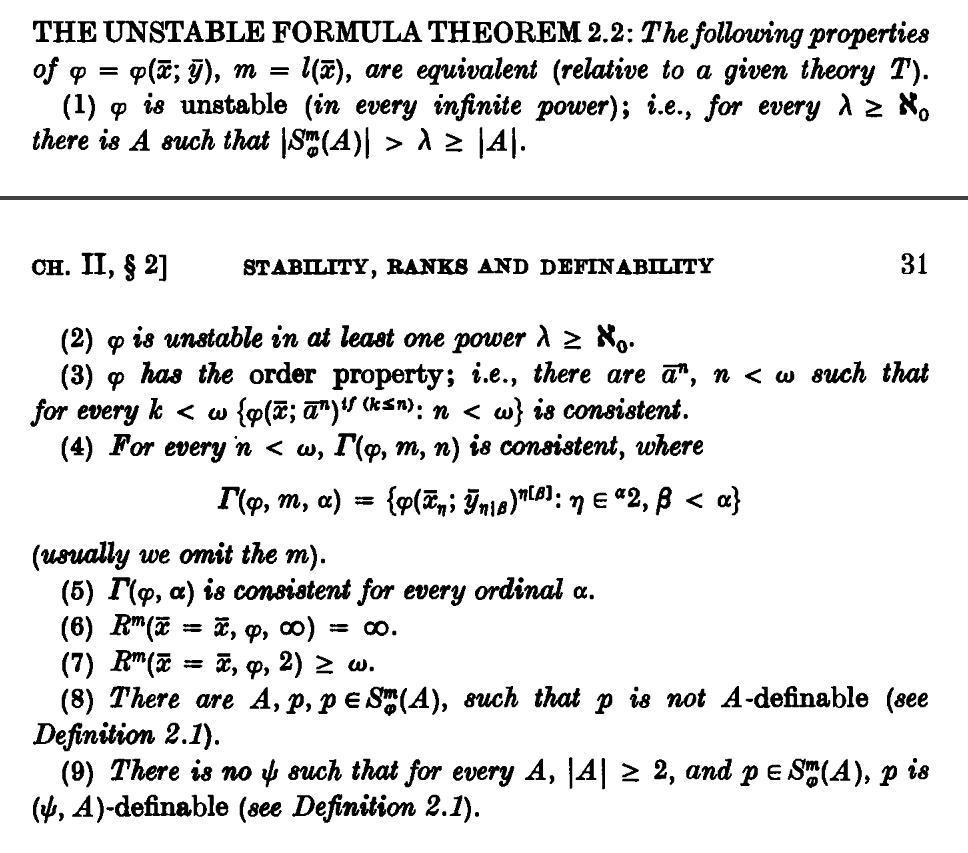
\includegraphics[width=\linewidth]{ShelahUnstable.png}
    \caption{The original statement of Shelah’s unstable formula theorem as it appears in \cite{Shelah1990}.}
    \label{fig:origStatement}
\end{figure}

\begin{fact}[The Unstable Formula Theorem $2.2$ in \cite{Shelah1990}]
\label{fact:unstableFormulaThm}
\begin{outline}
\0 For a formula $\phi$, the following properties are equivalent:
    \1 $\phi$ is stable,
    \1 $\shelahrank < \infty$ for any finite $\phi$-type $p$.
\end{outline}
\end{fact}

The proof of this theorem is quite lengthy, and draws from both model theory and combinatorics, introducing Stone spaces of complete $n$-types and going back to Ramsey and Erd\HH{o}s-Makkai theorem (so we omit it). Nonetheless this theorem allows us to show that stable theories are a subset of NIP theories, discussed in \cref{section:NIPtheories}.

\begin{theorem}
    Stable theories are NIP.
\end{theorem}
\begin{proof}
\begin{outline}
\contribution{3.}
\0 Let $T$ be a stable theory. Consider an arbitrary formula $\phi$ in $T$. Since $T$ is stable, $\phi$ is stable. We can establish that $\phi$ is NIP through the following chain of implications:
    \1[1)] The Shelah 2-rank of $\phi$ is finite (\cref{fact:unstableFormulaThm}).
    \1[2)] Finite Shelah 2-rank implies that the concept class $\C_\phi$ has finite Littlestone dimension (\cref{thm:LdimShelahRank}).
    \1[2)] Finite Littlestone dimension of $\C_\phi$ implies finite VC dimension of $\C_\phi$ (\cref{lemma:LdimboundsVC}).
    \1[3)] Finite VC dimension of $\C_\phi$ implies $\phi$ is NIP (\cref{thm:NIPfiniteVC}).
\0 Following this chain of implications, we conclude that $\phi$ is NIP. As $\phi$ was arbitrary, this holds for all formulas in $T$, therefore $T$ is NIP.
\end{outline}
\end{proof}

% What we do not omit, is a discussion of the parallels between it and \emph{algorithmic} version of the Unstable Formula Theorem. 

\begin{remark}
\contribution{1 --- Extended example from a discussion with Dr. Zou.}
    Given a class $\C_\phi$, there is a natural bipartite graph $G_\phi$ associated with any concept class. The node set of $G_\phi$ consists of two disjoint parts: the elements of the input set $X$ and the concepts in $\C_\phi$. We associate each concept $f\in\C_\phi$ with the parameter set $b_j$ defining it. The edge relation in $G_\phi$ is then defined by $\phi$. Specifically, there is an edge between $a_i\in X$ and $b_j\in\C_\phi$ if and only if $\phi(a_i;b_j)$ is true (or $f(a_i)=1$ if we view it as function in $\C_\phi$).
    This corresponds to the $k$-order-property we defined in \cref{def:stable}. The Littlestone dimension of $\C_\phi$ is finite if and only if there exists an upper bound on the size of any half-graph that appears as an induced subgraph of $G_\phi$. 
\end{remark}

We will now examine a number of examples of stable theories. They form a subclass of NIP theories and, as shown in \cref{section:fdmThmofPAC}, every formula $\phi$ in a stable theory has finite VC dimension. Consequently, it defines a PAC learnable concept class $\C_\phi$ with finite Littlestone dimension.

The strength of our approach is that it draws on the extensive work of model theorists over many decades. By linking stability to learnability, we gain access to a rich collection of examples that are known to be stable and thus learnable. Without model theory, direct proof of these properties is very difficult and intractable. 

Our exposition follows Section 5 in \cite{chase2019model}. For readers interested in a deeper exploration of these connections, we recommend consulting standard textbooks on model theory for more detailed treatments.

\begin{example}
\begin{outline}
\contribution{2 --- Worked out example with new additional details and connection to PAC learning.}
\0 The theory of algebraically closed fields ($\ACF$) is formulated in the ring signature $\cL_r=\{+,-,\cdot, 0,1\}$. It consists of the standard field axioms along with an infinite sequence of axioms, one for each positive integer $n$, stating that every polynomial of degree $n$ has a root: 

$$\phi_n = \forall y_0\ldots\forall y_{n-1} \exists x : x^n+\sum^{n-1}_{i=0} y_i x^i = 0.$$
    \1 $\ACF$ can be further specialized to describe fields of specific characteristic: 
        \2 For a prime $p$,  $\ACF_p$ is the theory of algebraically closed fields of characteristic $p$. It includes the additional axiom $\psi_p = \forall x : px = 0$, where $px$ denotes $x$ added to itself $p$ times.
        \2 For characteristic $0$,  $\ACF_0$ is the theory of algebraically closed fields of characteristic 0. It includes the negation of $\psi_p$ for all primes $p$, i.e., $\neg\psi_p = \exists x : px \neq 0$ for every prime $p$.

\0 Both $\ACF_0$ and $\ACF_p$ admit quantifier elimination. This allows any formula $\phi$ in these theories to be expressed as a quantifier-free formula, equivalent to a Boolean combination of polynomial equations and inequations.

\0 In the context of learning theory, for any formula $\phi$ in ACF, the corresponding concept class $\C_\phi$ is the solution set of this Boolean combination. In model-theoretic terms, this is a definable set (with parameters), while algebraic geometers refer to it as a constructible set. We can view this set as a subset of $\bA^n$, where $\bA$ is any algebraically closed field of the appropriate characteristic, and $n$ is the number of free variables in $\phi$.

\0 A concrete example of a concept class in this theory is the family of elliptic curves over the complex numbers, defined by the formula $\phi(x,y;a,b)=y^2=x^3+ax+b$, where $a$ and $b$ are parameters and $x$ and $y$ are variables. Given a set of points in $\C$, where each point is labeled based on whether it lies on a target elliptic curve, we can learn an approximation of that curve with high probability. The PAC learning guarantee ensures that with high probability, our learned curve will correctly classify most new points drawn from the same distribution as our training data.
\end{outline}
\end{example}

\begin{example}
\begin{outline}
\contribution{2 --- Worked out example with new additional details and connection to PAC learning.}
    \0 The second example is related to differential Galois theory. The theory of differentially closed fields in characteristic $0$ ($\DCF_0$) is formulated in the ring signature $\cL_r$ together with a unary function symbol $D$ dor the derivation. $\DCF_0$ consists of the axioms for $\ACF_0$, along with two axioms stating that $D$ is an additive homomorphism satisfying the product rule and one additional axiom: 
        \1 $\forall x,y: y D(x+y)=D(x)+D(y)$
        \1 $\forall x,y: y D(xy)=x D(y)+ yD(x)$
        \1 For any non-constant differential polynomials $p_1(x)$ and $p_2(x)$ of order $n_1 > n_2$ there is an $x$ such that $f(x)=0$ and $g(x)\neq 0$.
    \0 This last axiom is particularly important as it ensures that every consistent system of differential equations has a solution in the field. $\DCF_0$ admits quantifier elimination, allowing any formula $\phi$ in this theory to be expressed as a quantifier-free formula, equivalent to a Boolean combination of differential polynomial equations and inequations.
    
    A concrete example of a concept class in this theory is the family of solutions to linear differential equations, defined by the formula $\phi(y; a, b) = D(y) = ay + b$, where $a$ and $b$ are parameters and $y$ is a variable. Given a set of points in a differential field (e.g., the field of germs of meromorphic functions), where each point is labeled based on whether it satisfies a target linear differential equation, we can learn an approximation of that equation with high probability. 
\end{outline}
\end{example}

\begin{example}
\begin{outline}
\contribution{2 --- Worked out example with new additional details and connection to PAC learning.}
    \0 The third example comes from group theory. The elementary theory of a non-abelian free group $T_{fg}$, is formulated in the group signature $\cL_g = \{\cdot, ~^{-1}, 1\}$ and was shown to be stable by Zlil Sela in 2006. This theory cannot be axiomatized by first-order axioms, since the ultraproduct of free groups is not free. While this theory does not admit quantifier elimination, any formula in the language of groups is, modulo the theory of the free group, equivalent to a $\forall \exists$-formula. 
    
    A concrete example of a concept class in this theory could be the set of elements satisfying a certain word equation. For instance, we might consider $\phi(x;a,b)=x=aba^{-1}b^{-1}$, where $a$ and $b$ are parameters and $x$ is a variable. Given a set of elements in a free group, the stability of the theory guarantees that we can PAC learn the parameters $a$ and $b$ in this formula.
\end{outline}
\end{example}

\newpage

\section{Further Research}
\contribution{3 --- This section is completely original.}
In this thesis, we've proven the equivalence between finite VC dimension and NIP theories, finite Littlestone dimension and stable theories. This road opens up multiple ways to build upon these equivalences.

\begin{outline}
    \1 The reliance of both the Littlestone dimension and the VC dimension on shatter functions, which are themselves based on different forms of the Sauer-Shelah lemma, raises a question: Is there a unifying principle that encompasses both concepts?
    \marginnote[0cm]{\href{https://arxiv.org/abs/2203.12211}{arXiv:2203.12211v2, 2022}} This question is partially answered by Roland Walker in paper \enquote{Tree Dimension and the Sauer-Shelah Dichotomy} by defining a new tree dimension invariant called \emph{leveled tree dimension} to measure the complexity of leaf sets in binary trees.

    \1 The generalization to higher-arity trees has been explored by Hunter Chase and James Freitag in their paper \enquote{Model theory and combinatorics of banned sequences}. 
    \marginnote[0cm]{\href{https://arxiv.org/abs/1801.07640}{arXiv:1801.07640, 2018}} In this work, they study $2^s$-ary trees and apply it to the notion of model-theoretic $\ops$-rank introduced by Guingona and Hill. When $s=1$, this generalization recovers the original Shelah's 2-rank.

    \1 In the same paper, they address a question arising from the relationship between Littlestone dimension and VC dimension. Given that finite Littlestone dimension implies finite VC dimension, they investigate whether this stronger condition can lead to strengthening of the fundamental theorem of PAC learning. The authors provide a partial answer to this question by adapting the VC theorem to the context of finite Littlestone dimension. Their key contribution is showing that under these stronger assumptions, the VC theorem can be modified to allow for sampled elements to depend on the results of previous samples, in contrast to the independent sampling required in the standard VC theorem.

    \1 A connection to o-minimality comes from the fact that o-minimal theories are NIP. This can be used to show that if the activation functions of a neural network are definable in an o-minimal expansion of the real numbers (such as $\R_{\text{an,exp}}$, which includes analytic and exponential functions), then the hypothesis class computed by the network has finite VC dimension. This theoretical result has practical implications: it ensures that, given enough training samples, such neural networks can learn to approximate any concept to the best possible representation within their hypothesis class. A comprehensive reference on this topic is the textbook \enquote{Neural Network Learning: Theoretical Foundations} by Anthony and Bartlett. 

    \1 A more recent application of this concept was done by D'Inverno et al. in their paper \enquote{VC dimension of Graph Neural Networks with Pfaffian activation functions}. Their work extends this analysis to common GNN architectures. The authors derive upper bounds on the VC dimension in terms of key architectural parameters like the number of layers, hidden feature size, and input dimension. \marginnote[0cm]{\href{https://arxiv.org/abs/2401.12362}{arXiv:2401.12362v2, 2024}} They show that for GNNs with Pfaffian activations, the VC dimension grows as $O(p^4)$, where $p$ is the number of parameters. Theoretical results are supported by experiments measuring the gap between training and test accuracy as network size increases. 

    \1 The VC dimension is closely related to the concept of compression schemes. A classic example is compressing rectangles in $\R^2$ to just four points -- from an arbitrarily large set of labeled samples, one can select the four outermost positively labeled points and discard the rest. This compression retains all necessary information to recreate a labeling consistent with the full original sample, akin to the notion of sufficient statistics in probability and statistical theory. Just as sufficient statistics capture all relevant information about a parameter in a probabilistic model, these compression schemes encapsulate the essential information needed for learning.
    The now disproven Warmuth conjecture stated that every concept class of VC dimension at most $d$ admits a compression scheme of size at most $d$. \marginnote[0cm]{\href{https://arxiv.org/abs/1503.06960}{arXiv:1503.06960v2}, 2015\\~ \\
    \href{https://arxiv.org/abs/1811.12471}{arXiv:1811.12471v2, 2018}} Moran and Yehudayoff in \enquote{Sample compression schemes for VC classes} proved that there exists a compression scheme whose size is exponential in the VC dimension, and Pálvölgyi and Tardos in their paper \enquote{Unlabeled Compression Schemes Exceeding the VC-dimension} disproved this conjecture by constructing an explicit counterexample.
    
    \1 The uniform definability of types over finite sets (UDTFS) conjecture is another important model-theoretic conjecture that was recently proven by Eshel and Kaplan in their paper \enquote{On uniform definability of types over finite sets for NIP formulas}. \marginnote[0cm]{\href{https://arxiv.org/abs/1904.10336}{arXiv:1904.10336v2, 2020}} This conjecture states that a formula $\phi$ has the non-independence property (NIP) in a theory $T$ if and only if it has UDTFS in $T$. More specifically, UDTFS means that for any NIP formula $\phi$, there exists another formula $\phi$ that can uniformly define all possible $\phi$-types over any finite set of parameters.
    What's particularly interesting about the proof of this conjecture is that it combined two previously known results from machine learning theory. This is somewhat unusual, as typically model theory techniques are applied to machine learning problems rather than the reverse.
    
    \1 Last but certainly not least, the model theorists strike again. In paper \enquote{The Unstable Formula Theorem revisited via algorithms} Malliaris and Moran focused on developing a complete algorithmic analog of the Unstable Formula Theorem.\marginnote[0cm]{\href{https://arxiv.org/abs/2212.05050}{arXiv:2212.05050v2, 2023}} It summarizes all previous work on the subject and unifies it into one common framework. This provides a much clearer picture of the connections between model theory and machine learning. Furthermore, they also propose a new approach to online learning called \emph{probably eventually correct} learning (PEC) where the main difference between PEC and PAC learning is 
        \2 Error rate: 
            \3 PAC learning: The output hypothesis has low (but potentially non-zero) error with high probability.
            \3 PEC learning: The output hypothesis eventually has zero error (up to measure zero) with probability 1.
        \2 Sample complexity:
            \3 PAC learning: Requires a finite sample size to achieve the desired error/confidence.
            \3 PEC learning: Allows the sample size to be unbounded, only requiring the learner to eventually converge to the correct hypothesis.
        \2 Stability:
            \3 PAC learning: No explicit stability requirement on the output hypotheses.
            \3 PEC learning: Requires \emph{stable} learning in the sense that the algorithm changes its output hypothesis only a bounded number of times.
        \2 Algorithm:
            \3 PAC learning: No specific canonical algorithm.
            \3 PEC learning: The Standard Optimal Algorithm (SOA) is shown to be a PEC learner for Littlestone classes.
\end{outline}

\newpage 
\addcontentsline{toc}{section}{\protect\numberline{}References}
\printbibliography

\newpage 
\addcontentsline{toc}{section}{\protect\numberline{}Deutsche Zusammenfassung / German summary}
\section*{Deutsche Zusammenfassung / German summary}

\begin{outline}
\0 Die vorliegende Arbeit verfolgt das Ziel, die Zusammenhänge zwischen Modelltheorie und maschinellem Lernen an der Schnittstelle zwischen mathematischer Logik und Informatik zu beschreiben. Als Grundlage wurde der Artikel \enquote{Model Theory and Machine Learning} von Hunter und Chase verwendet, \cite{chase2019model}.

\begin{center}
\begin{tabular}{ c c c } 
$\{$Mathematische Logik$\}$ &  & ~$\{$Informatik$\}$ \\
$\bigcup$ & & ~$\bigcup$ \\
$\{$Modelltheorie$\}$ & $\bigcap$ & \quad~ $\{$Maschinelles Lernen$\}$
\end{tabular}
\end{center}

Wir konzentrieren uns dabei auf zwei zentrale Themenbereiche: Zum einen untersuchen wir die Verbindung zwischen PAC-Lernbarkeit und der NIP-Eigenschaft, zum anderen betrachten wir den Zusammenhang zwischen Online-Lernbarkeit und Stabilität. Beide Themen haben ihre Wurzeln in der Kombinatorik, ein Thema, das uns in den Beweisen immer wieder begleiten wird. Die Arbeit besteht aus zwei Hauptteilen:

Im ersten Teil beweisen wir das fundamentale Theorem der PAC-Lernbarkeit. Dieses besagt, dass eine Konzeptklasse genau dann PAC-lernbar ist, wenn sie eine endliche VC-Dimension hat. Auf der modelltheoretischen Seite wird anschließend die NIP-Eigenschaft eingeführt und gezeigt, dass Formeln in NIP-Theorien den Konzeptklassen mit endlicher VC-Dimension entsprechen.

Der zweite Teil widmet sich der Online-Lernbarkeit und der Littlestone-Dimension als Maß für die Komplexität einer Konzeptklasse. Wir stellen den Standard-Optimal-Algorithm als optimale Strategie für das Online-Lernen vor. Auf der modelltheoretischen Seite wird die Äquivalenz von endlicher Littlestone-Dimension und Shelahs 2-Rang, einem wichtigen Konzept aus der Modelltheorie, bewiesen. In Folge demonstrieren wir, dass Formeln in stabilen Theorien den Konzeptklassen mit endlicher Littlestone-Dimension entsprechen.

\begin{center}
\begin{tabular}{ c c c } 
endliche VC-Dimension & $\longleftrightarrow$ & NIP Theorie \\
$\bigcup$ & & $\bigcup$\\
endliche Littlestone-Dimension & $\longleftrightarrow$ & Stabile Theorie
\end{tabular}
\end{center}

Abschließend befassen wir uns mit der Stabilitätstheorie und zeigen, dass stabile Theorien eine Untermenge von NIP-Theorien bilden. Zur Veranschaulichung präsentieren wir mehrere Beispiele für stabile Theorien. Dazu gehören die Theorie algebraisch geschlossener Felder, die Theorie differenziell geschlossener Felder und die elementare Theorie nicht-abelscher freier Gruppen. Diese Beispiele demonstrieren, wie die Modelltheorie eine Vielzahl konkreter, PAC-lernbarer Konzeptklassen zum Vorschein bringt.
\end{outline}

\end{document}
